\documentclass{scrartcl}

    \usepackage{jupyterlatex}

    \usepackage[breakable]{tcolorbox}
    

    % Basic figure setup, for now with no caption control since it's done
    % automatically by Pandoc (which extracts ![](path) syntax from Markdown).
    \usepackage{graphicx}
    % Maintain compatibility with old templates. Remove in nbconvert 6.0
    \let\Oldincludegraphics\includegraphics
    % Ensure that by default, figures have no caption (until we provide a
    % proper Figure object with a Caption API and a way to capture that
    % in the conversion process - todo).
    \usepackage{caption}
    \DeclareCaptionFormat{nocaption}{}
    \captionsetup{format=nocaption,aboveskip=0pt,belowskip=0pt}

    \usepackage{float}
    \floatplacement{figure}{H} % forces figures to be placed at the correct location
    \usepackage{xcolor} % Allow colors to be defined
    \usepackage{enumerate} % Needed for markdown enumerations to work
    \usepackage{geometry} % Used to adjust the document margins
    \usepackage{amsmath} % Equations
    \usepackage{amssymb} % Equations
    \usepackage{textcomp} % defines textquotesingle
    % Hack from http://tex.stackexchange.com/a/47451/13684:
    \AtBeginDocument{%
        \def\PYZsq{\textquotesingle}% Upright quotes in Pygmentized code
    }
    \usepackage{upquote} % Upright quotes for verbatim code
    \usepackage{eurosym} % defines \euro

    \usepackage{iftex}
    \ifPDFTeX
        \usepackage[T1]{fontenc}
        \IfFileExists{alphabeta.sty}{
              \usepackage{alphabeta}
          }{
              \usepackage[mathletters]{ucs}
              \usepackage[utf8]{inputenc}
          }
    \else
        \usepackage{fontspec}
        \usepackage{unicode-math}
    \fi

    \usepackage{fancyvrb} % verbatim replacement that allows latex
    \usepackage{grffile} % extends the file name processing of package graphics 
                         % to support a larger range
    \makeatletter % fix for old versions of grffile with XeLaTeX
    \@ifpackagelater{grffile}{2019/11/01}
    {
      % Do nothing on new versions
    }
    {
      \def\Gread@@xetex#1{%
        \IfFileExists{"\Gin@base".bb}%
        {\Gread@eps{\Gin@base.bb}}%
        {\Gread@@xetex@aux#1}%
      }
    }
    \makeatother
    \usepackage[Export]{adjustbox} % Used to constrain images to a maximum size
    \adjustboxset{max size={0.9\linewidth}{0.9\paperheight}}

    % The hyperref package gives us a pdf with properly built
    % internal navigation ('pdf bookmarks' for the table of contents,
    % internal cross-reference links, web links for URLs, etc.)
    \usepackage{hyperref}
    % The default LaTeX title has an obnoxious amount of whitespace. By default,
    % titling removes some of it. It also provides customization options.
    \usepackage{longtable} % longtable support required by pandoc >1.10
    \usepackage{booktabs}  % table support for pandoc > 1.12.2
    \usepackage{array}     % table support for pandoc >= 2.11.3
    \usepackage{calc}      % table minipage width calculation for pandoc >= 2.11.1
    \usepackage[inline]{enumitem} % IRkernel/repr support (it uses the enumerate* environment)
    \usepackage[normalem]{ulem} % ulem is needed to support strikethroughs (\sout)
                                % normalem makes italics be italics, not underlines
    \usepackage{mathrsfs}
    

    
    % Colors for the hyperref package
    \definecolor{urlcolor}{rgb}{0,.145,.698}
    \definecolor{linkcolor}{rgb}{.71,0.21,0.01}
    \definecolor{citecolor}{rgb}{.12,.54,.11}

    % ANSI colors
    \definecolor{ansi-black}{HTML}{3E424D}
    \definecolor{ansi-black-intense}{HTML}{282C36}
    \definecolor{ansi-red}{HTML}{E75C58}
    \definecolor{ansi-red-intense}{HTML}{B22B31}
    \definecolor{ansi-green}{HTML}{00A250}
    \definecolor{ansi-green-intense}{HTML}{007427}
    \definecolor{ansi-yellow}{HTML}{DDB62B}
    \definecolor{ansi-yellow-intense}{HTML}{B27D12}
    \definecolor{ansi-blue}{HTML}{208FFB}
    \definecolor{ansi-blue-intense}{HTML}{0065CA}
    \definecolor{ansi-magenta}{HTML}{D160C4}
    \definecolor{ansi-magenta-intense}{HTML}{A03196}
    \definecolor{ansi-cyan}{HTML}{60C6C8}
    \definecolor{ansi-cyan-intense}{HTML}{258F8F}
    \definecolor{ansi-white}{HTML}{C5C1B4}
    \definecolor{ansi-white-intense}{HTML}{A1A6B2}
    \definecolor{ansi-default-inverse-fg}{HTML}{FFFFFF}
    \definecolor{ansi-default-inverse-bg}{HTML}{000000}

    % common color for the border for error outputs.
    \definecolor{outerrorbackground}{HTML}{FFDFDF}

    % commands and environments needed by pandoc snippets
    % extracted from the output of `pandoc -s`
    \providecommand{\tightlist}{%
      \setlength{\itemsep}{0pt}\setlength{\parskip}{0pt}}
    \DefineVerbatimEnvironment{Highlighting}{Verbatim}{commandchars=\\\{\}}
    % Add ',fontsize=\small' for more characters per line
    \newenvironment{Shaded}{}{}
    \newcommand{\KeywordTok}[1]{\textcolor[rgb]{0.00,0.44,0.13}{\textbf{{#1}}}}
    \newcommand{\DataTypeTok}[1]{\textcolor[rgb]{0.56,0.13,0.00}{{#1}}}
    \newcommand{\DecValTok}[1]{\textcolor[rgb]{0.25,0.63,0.44}{{#1}}}
    \newcommand{\BaseNTok}[1]{\textcolor[rgb]{0.25,0.63,0.44}{{#1}}}
    \newcommand{\FloatTok}[1]{\textcolor[rgb]{0.25,0.63,0.44}{{#1}}}
    \newcommand{\CharTok}[1]{\textcolor[rgb]{0.25,0.44,0.63}{{#1}}}
    \newcommand{\StringTok}[1]{\textcolor[rgb]{0.25,0.44,0.63}{{#1}}}
    \newcommand{\CommentTok}[1]{\textcolor[rgb]{0.38,0.63,0.69}{\textit{{#1}}}}
    \newcommand{\OtherTok}[1]{\textcolor[rgb]{0.00,0.44,0.13}{{#1}}}
    \newcommand{\AlertTok}[1]{\textcolor[rgb]{1.00,0.00,0.00}{\textbf{{#1}}}}
    \newcommand{\FunctionTok}[1]{\textcolor[rgb]{0.02,0.16,0.49}{{#1}}}
    \newcommand{\RegionMarkerTok}[1]{{#1}}
    \newcommand{\ErrorTok}[1]{\textcolor[rgb]{1.00,0.00,0.00}{\textbf{{#1}}}}
    \newcommand{\NormalTok}[1]{{#1}}
    
    % Additional commands for more recent versions of Pandoc
    \newcommand{\ConstantTok}[1]{\textcolor[rgb]{0.53,0.00,0.00}{{#1}}}
    \newcommand{\SpecialCharTok}[1]{\textcolor[rgb]{0.25,0.44,0.63}{{#1}}}
    \newcommand{\VerbatimStringTok}[1]{\textcolor[rgb]{0.25,0.44,0.63}{{#1}}}
    \newcommand{\SpecialStringTok}[1]{\textcolor[rgb]{0.73,0.40,0.53}{{#1}}}
    \newcommand{\ImportTok}[1]{{#1}}
    \newcommand{\DocumentationTok}[1]{\textcolor[rgb]{0.73,0.13,0.13}{\textit{{#1}}}}
    \newcommand{\AnnotationTok}[1]{\textcolor[rgb]{0.38,0.63,0.69}{\textbf{\textit{{#1}}}}}
    \newcommand{\CommentVarTok}[1]{\textcolor[rgb]{0.38,0.63,0.69}{\textbf{\textit{{#1}}}}}
    \newcommand{\VariableTok}[1]{\textcolor[rgb]{0.10,0.09,0.49}{{#1}}}
    \newcommand{\ControlFlowTok}[1]{\textcolor[rgb]{0.00,0.44,0.13}{\textbf{{#1}}}}
    \newcommand{\OperatorTok}[1]{\textcolor[rgb]{0.40,0.40,0.40}{{#1}}}
    \newcommand{\BuiltInTok}[1]{{#1}}
    \newcommand{\ExtensionTok}[1]{{#1}}
    \newcommand{\PreprocessorTok}[1]{\textcolor[rgb]{0.74,0.48,0.00}{{#1}}}
    \newcommand{\AttributeTok}[1]{\textcolor[rgb]{0.49,0.56,0.16}{{#1}}}
    \newcommand{\InformationTok}[1]{\textcolor[rgb]{0.38,0.63,0.69}{\textbf{\textit{{#1}}}}}
    \newcommand{\WarningTok}[1]{\textcolor[rgb]{0.38,0.63,0.69}{\textbf{\textit{{#1}}}}}
    
    
    % Define a nice break command that doesn't care if a line doesn't already
    % exist.
    \def\br{\hspace*{\fill} \\* }
    % Math Jax compatibility definitions
    \def\gt{>}
    \def\lt{<}
    \let\Oldtex\TeX
    \let\Oldlatex\LaTeX
    \renewcommand{\TeX}{\textrm{\Oldtex}}
    \renewcommand{\LaTeX}{\textrm{\Oldlatex}}
    % Document parameters
    % Document title
    \newcommand*{\mytitle}{Unit 8: Data input and output}

    % Included at the bottom of the preamble

\usepackage{microtype}


\title{\mytitle}
\author{Richard Foltyn}
\hypersetup{pdfauthor={Richard Foltyn}, pdftitle={\mytitle}}

% Remove horizontal rules in a very hackish way
\renewcommand{\rule}[2]{}

\RequirePackage{xspace}


\newcommand*{\eg}{e.g.\@\xspace}
\newcommand*{\Eg}{E.g.\@\xspace}
\newcommand*{\etc}{etc.\@\xspace}
\newcommand*{\ie}{i.e.\@\xspace}
\newcommand*{\vs}{vs.\@\xspace}
\newcommand*{\viz}{viz.\@\xspace}
\newcommand*{\US}{U.S.\@\xspace}

    
    
    
    
    
% Pygments definitions
\makeatletter
\def\PY@reset{\let\PY@it=\relax \let\PY@bf=\relax%
    \let\PY@ul=\relax \let\PY@tc=\relax%
    \let\PY@bc=\relax \let\PY@ff=\relax}
\def\PY@tok#1{\csname PY@tok@#1\endcsname}
\def\PY@toks#1+{\ifx\relax#1\empty\else%
    \PY@tok{#1}\expandafter\PY@toks\fi}
\def\PY@do#1{\PY@bc{\PY@tc{\PY@ul{%
    \PY@it{\PY@bf{\PY@ff{#1}}}}}}}
\def\PY#1#2{\PY@reset\PY@toks#1+\relax+\PY@do{#2}}

\@namedef{PY@tok@w}{\def\PY@tc##1{\textcolor[rgb]{0.73,0.73,0.73}{##1}}}
\@namedef{PY@tok@c}{\let\PY@it=\textit\def\PY@tc##1{\textcolor[rgb]{0.24,0.48,0.48}{##1}}}
\@namedef{PY@tok@cp}{\def\PY@tc##1{\textcolor[rgb]{0.61,0.40,0.00}{##1}}}
\@namedef{PY@tok@k}{\let\PY@bf=\textbf\def\PY@tc##1{\textcolor[rgb]{0.00,0.50,0.00}{##1}}}
\@namedef{PY@tok@kp}{\def\PY@tc##1{\textcolor[rgb]{0.00,0.50,0.00}{##1}}}
\@namedef{PY@tok@kt}{\def\PY@tc##1{\textcolor[rgb]{0.69,0.00,0.25}{##1}}}
\@namedef{PY@tok@o}{\def\PY@tc##1{\textcolor[rgb]{0.40,0.40,0.40}{##1}}}
\@namedef{PY@tok@ow}{\let\PY@bf=\textbf\def\PY@tc##1{\textcolor[rgb]{0.67,0.13,1.00}{##1}}}
\@namedef{PY@tok@nb}{\def\PY@tc##1{\textcolor[rgb]{0.00,0.50,0.00}{##1}}}
\@namedef{PY@tok@nf}{\def\PY@tc##1{\textcolor[rgb]{0.00,0.00,1.00}{##1}}}
\@namedef{PY@tok@nc}{\let\PY@bf=\textbf\def\PY@tc##1{\textcolor[rgb]{0.00,0.00,1.00}{##1}}}
\@namedef{PY@tok@nn}{\let\PY@bf=\textbf\def\PY@tc##1{\textcolor[rgb]{0.00,0.00,1.00}{##1}}}
\@namedef{PY@tok@ne}{\let\PY@bf=\textbf\def\PY@tc##1{\textcolor[rgb]{0.80,0.25,0.22}{##1}}}
\@namedef{PY@tok@nv}{\def\PY@tc##1{\textcolor[rgb]{0.10,0.09,0.49}{##1}}}
\@namedef{PY@tok@no}{\def\PY@tc##1{\textcolor[rgb]{0.53,0.00,0.00}{##1}}}
\@namedef{PY@tok@nl}{\def\PY@tc##1{\textcolor[rgb]{0.46,0.46,0.00}{##1}}}
\@namedef{PY@tok@ni}{\let\PY@bf=\textbf\def\PY@tc##1{\textcolor[rgb]{0.44,0.44,0.44}{##1}}}
\@namedef{PY@tok@na}{\def\PY@tc##1{\textcolor[rgb]{0.41,0.47,0.13}{##1}}}
\@namedef{PY@tok@nt}{\let\PY@bf=\textbf\def\PY@tc##1{\textcolor[rgb]{0.00,0.50,0.00}{##1}}}
\@namedef{PY@tok@nd}{\def\PY@tc##1{\textcolor[rgb]{0.67,0.13,1.00}{##1}}}
\@namedef{PY@tok@s}{\def\PY@tc##1{\textcolor[rgb]{0.73,0.13,0.13}{##1}}}
\@namedef{PY@tok@sd}{\let\PY@it=\textit\def\PY@tc##1{\textcolor[rgb]{0.73,0.13,0.13}{##1}}}
\@namedef{PY@tok@si}{\let\PY@bf=\textbf\def\PY@tc##1{\textcolor[rgb]{0.64,0.35,0.47}{##1}}}
\@namedef{PY@tok@se}{\let\PY@bf=\textbf\def\PY@tc##1{\textcolor[rgb]{0.67,0.36,0.12}{##1}}}
\@namedef{PY@tok@sr}{\def\PY@tc##1{\textcolor[rgb]{0.64,0.35,0.47}{##1}}}
\@namedef{PY@tok@ss}{\def\PY@tc##1{\textcolor[rgb]{0.10,0.09,0.49}{##1}}}
\@namedef{PY@tok@sx}{\def\PY@tc##1{\textcolor[rgb]{0.00,0.50,0.00}{##1}}}
\@namedef{PY@tok@m}{\def\PY@tc##1{\textcolor[rgb]{0.40,0.40,0.40}{##1}}}
\@namedef{PY@tok@gh}{\let\PY@bf=\textbf\def\PY@tc##1{\textcolor[rgb]{0.00,0.00,0.50}{##1}}}
\@namedef{PY@tok@gu}{\let\PY@bf=\textbf\def\PY@tc##1{\textcolor[rgb]{0.50,0.00,0.50}{##1}}}
\@namedef{PY@tok@gd}{\def\PY@tc##1{\textcolor[rgb]{0.63,0.00,0.00}{##1}}}
\@namedef{PY@tok@gi}{\def\PY@tc##1{\textcolor[rgb]{0.00,0.52,0.00}{##1}}}
\@namedef{PY@tok@gr}{\def\PY@tc##1{\textcolor[rgb]{0.89,0.00,0.00}{##1}}}
\@namedef{PY@tok@ge}{\let\PY@it=\textit}
\@namedef{PY@tok@gs}{\let\PY@bf=\textbf}
\@namedef{PY@tok@gp}{\let\PY@bf=\textbf\def\PY@tc##1{\textcolor[rgb]{0.00,0.00,0.50}{##1}}}
\@namedef{PY@tok@go}{\def\PY@tc##1{\textcolor[rgb]{0.44,0.44,0.44}{##1}}}
\@namedef{PY@tok@gt}{\def\PY@tc##1{\textcolor[rgb]{0.00,0.27,0.87}{##1}}}
\@namedef{PY@tok@err}{\def\PY@bc##1{{\setlength{\fboxsep}{\string -\fboxrule}\fcolorbox[rgb]{1.00,0.00,0.00}{1,1,1}{\strut ##1}}}}
\@namedef{PY@tok@kc}{\let\PY@bf=\textbf\def\PY@tc##1{\textcolor[rgb]{0.00,0.50,0.00}{##1}}}
\@namedef{PY@tok@kd}{\let\PY@bf=\textbf\def\PY@tc##1{\textcolor[rgb]{0.00,0.50,0.00}{##1}}}
\@namedef{PY@tok@kn}{\let\PY@bf=\textbf\def\PY@tc##1{\textcolor[rgb]{0.00,0.50,0.00}{##1}}}
\@namedef{PY@tok@kr}{\let\PY@bf=\textbf\def\PY@tc##1{\textcolor[rgb]{0.00,0.50,0.00}{##1}}}
\@namedef{PY@tok@bp}{\def\PY@tc##1{\textcolor[rgb]{0.00,0.50,0.00}{##1}}}
\@namedef{PY@tok@fm}{\def\PY@tc##1{\textcolor[rgb]{0.00,0.00,1.00}{##1}}}
\@namedef{PY@tok@vc}{\def\PY@tc##1{\textcolor[rgb]{0.10,0.09,0.49}{##1}}}
\@namedef{PY@tok@vg}{\def\PY@tc##1{\textcolor[rgb]{0.10,0.09,0.49}{##1}}}
\@namedef{PY@tok@vi}{\def\PY@tc##1{\textcolor[rgb]{0.10,0.09,0.49}{##1}}}
\@namedef{PY@tok@vm}{\def\PY@tc##1{\textcolor[rgb]{0.10,0.09,0.49}{##1}}}
\@namedef{PY@tok@sa}{\def\PY@tc##1{\textcolor[rgb]{0.73,0.13,0.13}{##1}}}
\@namedef{PY@tok@sb}{\def\PY@tc##1{\textcolor[rgb]{0.73,0.13,0.13}{##1}}}
\@namedef{PY@tok@sc}{\def\PY@tc##1{\textcolor[rgb]{0.73,0.13,0.13}{##1}}}
\@namedef{PY@tok@dl}{\def\PY@tc##1{\textcolor[rgb]{0.73,0.13,0.13}{##1}}}
\@namedef{PY@tok@s2}{\def\PY@tc##1{\textcolor[rgb]{0.73,0.13,0.13}{##1}}}
\@namedef{PY@tok@sh}{\def\PY@tc##1{\textcolor[rgb]{0.73,0.13,0.13}{##1}}}
\@namedef{PY@tok@s1}{\def\PY@tc##1{\textcolor[rgb]{0.73,0.13,0.13}{##1}}}
\@namedef{PY@tok@mb}{\def\PY@tc##1{\textcolor[rgb]{0.40,0.40,0.40}{##1}}}
\@namedef{PY@tok@mf}{\def\PY@tc##1{\textcolor[rgb]{0.40,0.40,0.40}{##1}}}
\@namedef{PY@tok@mh}{\def\PY@tc##1{\textcolor[rgb]{0.40,0.40,0.40}{##1}}}
\@namedef{PY@tok@mi}{\def\PY@tc##1{\textcolor[rgb]{0.40,0.40,0.40}{##1}}}
\@namedef{PY@tok@il}{\def\PY@tc##1{\textcolor[rgb]{0.40,0.40,0.40}{##1}}}
\@namedef{PY@tok@mo}{\def\PY@tc##1{\textcolor[rgb]{0.40,0.40,0.40}{##1}}}
\@namedef{PY@tok@ch}{\let\PY@it=\textit\def\PY@tc##1{\textcolor[rgb]{0.24,0.48,0.48}{##1}}}
\@namedef{PY@tok@cm}{\let\PY@it=\textit\def\PY@tc##1{\textcolor[rgb]{0.24,0.48,0.48}{##1}}}
\@namedef{PY@tok@cpf}{\let\PY@it=\textit\def\PY@tc##1{\textcolor[rgb]{0.24,0.48,0.48}{##1}}}
\@namedef{PY@tok@c1}{\let\PY@it=\textit\def\PY@tc##1{\textcolor[rgb]{0.24,0.48,0.48}{##1}}}
\@namedef{PY@tok@cs}{\let\PY@it=\textit\def\PY@tc##1{\textcolor[rgb]{0.24,0.48,0.48}{##1}}}

\def\PYZbs{\char`\\}
\def\PYZus{\char`\_}
\def\PYZob{\char`\{}
\def\PYZcb{\char`\}}
\def\PYZca{\char`\^}
\def\PYZam{\char`\&}
\def\PYZlt{\char`\<}
\def\PYZgt{\char`\>}
\def\PYZsh{\char`\#}
\def\PYZpc{\char`\%}
\def\PYZdl{\char`\$}
\def\PYZhy{\char`\-}
\def\PYZsq{\char`\'}
\def\PYZdq{\char`\"}
\def\PYZti{\char`\~}
% for compatibility with earlier versions
\def\PYZat{@}
\def\PYZlb{[}
\def\PYZrb{]}
\makeatother


    % For linebreaks inside Verbatim environment from package fancyvrb. 
    \makeatletter
        \newbox\Wrappedcontinuationbox 
        \newbox\Wrappedvisiblespacebox 
        \newcommand*\Wrappedvisiblespace {\textcolor{red}{\textvisiblespace}} 
        \newcommand*\Wrappedcontinuationsymbol {\textcolor{red}{\llap{\tiny$\m@th\hookrightarrow$}}} 
        \newcommand*\Wrappedcontinuationindent {3ex } 
        \newcommand*\Wrappedafterbreak {\kern\Wrappedcontinuationindent\copy\Wrappedcontinuationbox} 
        % Take advantage of the already applied Pygments mark-up to insert 
        % potential linebreaks for TeX processing. 
        %        {, <, #, %, $, ' and ": go to next line. 
        %        _, }, ^, &, >, - and ~: stay at end of broken line. 
        % Use of \textquotesingle for straight quote. 
        \newcommand*\Wrappedbreaksatspecials {% 
            \def\PYGZus{\discretionary{\char`\_}{\Wrappedafterbreak}{\char`\_}}% 
            \def\PYGZob{\discretionary{}{\Wrappedafterbreak\char`\{}{\char`\{}}% 
            \def\PYGZcb{\discretionary{\char`\}}{\Wrappedafterbreak}{\char`\}}}% 
            \def\PYGZca{\discretionary{\char`\^}{\Wrappedafterbreak}{\char`\^}}% 
            \def\PYGZam{\discretionary{\char`\&}{\Wrappedafterbreak}{\char`\&}}% 
            \def\PYGZlt{\discretionary{}{\Wrappedafterbreak\char`\<}{\char`\<}}% 
            \def\PYGZgt{\discretionary{\char`\>}{\Wrappedafterbreak}{\char`\>}}% 
            \def\PYGZsh{\discretionary{}{\Wrappedafterbreak\char`\#}{\char`\#}}% 
            \def\PYGZpc{\discretionary{}{\Wrappedafterbreak\char`\%}{\char`\%}}% 
            \def\PYGZdl{\discretionary{}{\Wrappedafterbreak\char`\$}{\char`\$}}% 
            \def\PYGZhy{\discretionary{\char`\-}{\Wrappedafterbreak}{\char`\-}}% 
            \def\PYGZsq{\discretionary{}{\Wrappedafterbreak\textquotesingle}{\textquotesingle}}% 
            \def\PYGZdq{\discretionary{}{\Wrappedafterbreak\char`\"}{\char`\"}}% 
            \def\PYGZti{\discretionary{\char`\~}{\Wrappedafterbreak}{\char`\~}}% 
        } 
        % Some characters . , ; ? ! / are not pygmentized. 
        % This macro makes them "active" and they will insert potential linebreaks 
        \newcommand*\Wrappedbreaksatpunct {% 
            \lccode`\~`\.\lowercase{\def~}{\discretionary{\hbox{\char`\.}}{\Wrappedafterbreak}{\hbox{\char`\.}}}% 
            \lccode`\~`\,\lowercase{\def~}{\discretionary{\hbox{\char`\,}}{\Wrappedafterbreak}{\hbox{\char`\,}}}% 
            \lccode`\~`\;\lowercase{\def~}{\discretionary{\hbox{\char`\;}}{\Wrappedafterbreak}{\hbox{\char`\;}}}% 
            \lccode`\~`\:\lowercase{\def~}{\discretionary{\hbox{\char`\:}}{\Wrappedafterbreak}{\hbox{\char`\:}}}% 
            \lccode`\~`\?\lowercase{\def~}{\discretionary{\hbox{\char`\?}}{\Wrappedafterbreak}{\hbox{\char`\?}}}% 
            \lccode`\~`\!\lowercase{\def~}{\discretionary{\hbox{\char`\!}}{\Wrappedafterbreak}{\hbox{\char`\!}}}% 
            \lccode`\~`\/\lowercase{\def~}{\discretionary{\hbox{\char`\/}}{\Wrappedafterbreak}{\hbox{\char`\/}}}% 
            \catcode`\.\active
            \catcode`\,\active 
            \catcode`\;\active
            \catcode`\:\active
            \catcode`\?\active
            \catcode`\!\active
            \catcode`\/\active 
            \lccode`\~`\~ 	
        }
    \makeatother

    \let\OriginalVerbatim=\Verbatim
    \makeatletter
    \renewcommand{\Verbatim}[1][1]{%
        %\parskip\z@skip
        \sbox\Wrappedcontinuationbox {\Wrappedcontinuationsymbol}%
        \sbox\Wrappedvisiblespacebox {\FV@SetupFont\Wrappedvisiblespace}%
        \def\FancyVerbFormatLine ##1{\hsize\linewidth
            \vtop{\raggedright\hyphenpenalty\z@\exhyphenpenalty\z@
                \doublehyphendemerits\z@\finalhyphendemerits\z@
                \strut ##1\strut}%
        }%
        % If the linebreak is at a space, the latter will be displayed as visible
        % space at end of first line, and a continuation symbol starts next line.
        % Stretch/shrink are however usually zero for typewriter font.
        \def\FV@Space {%
            \nobreak\hskip\z@ plus\fontdimen3\font minus\fontdimen4\font
            \discretionary{\copy\Wrappedvisiblespacebox}{\Wrappedafterbreak}
            {\kern\fontdimen2\font}%
        }%
        
        % Allow breaks at special characters using \PYG... macros.
        \Wrappedbreaksatspecials
        % Breaks at punctuation characters . , ; ? ! and / need catcode=\active 	
        \OriginalVerbatim[#1,fontsize=\small,codes*=\Wrappedbreaksatpunct]%
    }
    \makeatother

    % Exact colors from NB
    \definecolor{incolor}{HTML}{303F9F}
    \definecolor{outcolor}{HTML}{D84315}
    \definecolor{cellborder}{HTML}{CFCFCF}
    \definecolor{cellbackground}{HTML}{FCFCFC}
    
    % prompt
    \makeatletter
    \newcommand{\boxspacing}{\kern\kvtcb@left@rule\kern\kvtcb@boxsep}
    \makeatother
    \newcommand{\prompt}[4]{
        {\ttfamily\llap{{\color{#2}[#3]:\hspace{3pt}#4}}\vspace{-\baselineskip}}
    }
    

    
    % Prevent overflowing lines due to hard-to-break entities
    \sloppy 
    % Setup hyperref package
    \hypersetup{
      breaklinks=true,  % so long urls are correctly broken across lines
      colorlinks=true,
      urlcolor=urlcolor,
      linkcolor=linkcolor,
      citecolor=citecolor,
      }
    % Slightly bigger margins than the latex defaults
    
    \geometry{verbose,tmargin=1in,bmargin=1in,lmargin=1in,rmargin=1in}
    
    

\begin{document}
    
    \maketitle
    \tableofcontents
    
    

    
    \hypertarget{data-input-and-output}{%
\section{Data input and output}\label{data-input-and-output}}

In this unit we discuss input and output, or I/O for short. We focus
exclusively on I/O routines used to load and store data from files that
are relevant for numerical computation and data analysis.

    \hypertarget{io-with-numpy}{%
\subsection{I/O with NumPy}\label{io-with-numpy}}

\hypertarget{loading-text-data}{%
\subsubsection{Loading text data}\label{loading-text-data}}

We have already encountered the most basic, and probably most frequently
used NumPy I/O routine, \texttt{np.loadtxt()}. We often use files that
store data as text files containing character-separated values (CSV)
since virtually any application supports this data format. The most
important I/O functions to process text data are:

\begin{itemize}
\tightlist
\item
  \href{https://numpy.org/doc/stable/reference/generated/numpy.loadtxt.html}{\texttt{np.loadtxt()}}:
  load data from a text file.
\item
  \href{https://numpy.org/doc/stable/reference/generated/numpy.genfromtxt.html}{\texttt{np.genfromtxt()}}:
  load data from a text file and handle missing data.
\item
  \href{https://numpy.org/doc/stable/reference/generated/numpy.savetxt.html}{\texttt{np.savetxt()}}:
  save a NumPy array to a text file.
\end{itemize}

There are a few other I/O functions in NumPy, for example to write
arrays as raw binary data. We won't cover them here, but you can find
them in the
\href{https://numpy.org/doc/stable/reference/routines.io.html}{official
documentation}.

Imagine we have the following tabular data from
\href{https://fred.stlouisfed.org/}{FRED}, where the first two rows look
as follows:

\begin{longtable}[]{@{}llll@{}}
\toprule
Year & GDP & CPI & UNRATE\tabularnewline
\midrule
\endhead
1948 & 2118.5 & 24.0 & 3.8\tabularnewline
1949 & 2106.6 & 23.8 & 6.0\tabularnewline
\bottomrule
\end{longtable}

To load this CSV file as a NumPy array, we use \texttt{loadtxt()}. As in
the previous unit, it is advantageous to globally set the path to the
\texttt{data/} directory that can point either to the local directory or
to the \texttt{data/} directory on GitHub.

    \begin{tcolorbox}[breakable, size=fbox, boxrule=1pt, pad at break*=1mm,colback=cellbackground, colframe=cellborder]
\prompt{In}{incolor}{1}{\boxspacing}
\begin{Verbatim}[commandchars=\\\{\}]
\PY{c+c1}{\PYZsh{} Uncomment this to use files in the local data/ directory}
\PY{c+c1}{\PYZsh{} DATA\PYZus{}PATH = \PYZsq{}../data\PYZsq{}}

\PY{c+c1}{\PYZsh{} Load data directly from GitHub}
\PY{n}{DATA\PYZus{}PATH} \PY{o}{=} \PY{l+s+s1}{\PYZsq{}}\PY{l+s+s1}{https://raw.githubusercontent.com/richardfoltyn/MLFP\PYZhy{}ECON5130/main/data}\PY{l+s+s1}{\PYZsq{}}
\end{Verbatim}
\end{tcolorbox}

    \begin{tcolorbox}[breakable, size=fbox, boxrule=1pt, pad at break*=1mm,colback=cellbackground, colframe=cellborder]
\prompt{In}{incolor}{2}{\boxspacing}
\begin{Verbatim}[commandchars=\\\{\}]
\PY{k+kn}{import} \PY{n+nn}{numpy} \PY{k}{as} \PY{n+nn}{np}


\PY{c+c1}{\PYZsh{} relative path to CSV file}
\PY{n}{file} \PY{o}{=} \PY{l+s+sa}{f}\PY{l+s+s1}{\PYZsq{}}\PY{l+s+si}{\PYZob{}}\PY{n}{DATA\PYZus{}PATH}\PY{l+s+si}{\PYZcb{}}\PY{l+s+s1}{/FRED.csv}\PY{l+s+s1}{\PYZsq{}}

\PY{c+c1}{\PYZsh{} load CSV}
\PY{n}{data} \PY{o}{=} \PY{n}{np}\PY{o}{.}\PY{n}{loadtxt}\PY{p}{(}\PY{n}{file}\PY{p}{,} \PY{n}{skiprows}\PY{o}{=}\PY{l+m+mi}{1}\PY{p}{,} \PY{n}{delimiter}\PY{o}{=}\PY{l+s+s1}{\PYZsq{}}\PY{l+s+s1}{,}\PY{l+s+s1}{\PYZsq{}}\PY{p}{)}
\PY{n}{data}\PY{p}{[}\PY{p}{:}\PY{l+m+mi}{2}\PY{p}{]}        \PY{c+c1}{\PYZsh{} Display first two rows}
\end{Verbatim}
\end{tcolorbox}

            \begin{tcolorbox}[breakable, size=fbox, boxrule=.5pt, pad at break*=1mm, opacityfill=0]
\prompt{Out}{outcolor}{2}{\boxspacing}
\begin{Verbatim}[commandchars=\\\{\}]
array([[1948. , 2118.5,   24. ,    3.8],
       [1949. , 2106.6,   23.8,    6. ]])
\end{Verbatim}
\end{tcolorbox}
        
    The default settings will in many cases be appropriate to load whatever
CSV file we might have. However, we'll occasionally want to specify the
following arguments to override the defaults:

\begin{itemize}
\tightlist
\item
  \texttt{delimiter}: Character used to separate individual fields
  (default: space).
\item
  \texttt{skiprows=n}: Skip the first \texttt{n} rows. For example, if
  the CSV file contains a header with variable names,
  \texttt{skiprows=1} needs to be specified as NumPy by default cannot
  process these names.
\item
  \texttt{dtype}: Enforce a particular data type for the resulting
  array.
\item
  \texttt{encoding}: Set the character encoding of the input data. This
  is usually not needed, but can be required to import data with
  non-latin characters that are not encoded using Unicode.
\end{itemize}

While \texttt{loadtxt()} is simple to use, it quickly reaches its limits
with more complex data sets. For example, when we try to load our sample
of universities with \texttt{loadtxt()}, we get the following error:

    \begin{tcolorbox}[breakable, size=fbox, boxrule=1pt, pad at break*=1mm,colback=cellbackground, colframe=cellborder]
\prompt{In}{incolor}{3}{\boxspacing}
\begin{Verbatim}[commandchars=\\\{\}]
\PY{k+kn}{import} \PY{n+nn}{numpy} \PY{k}{as} \PY{n+nn}{np}

\PY{n}{file} \PY{o}{=} \PY{l+s+sa}{f}\PY{l+s+s1}{\PYZsq{}}\PY{l+s+si}{\PYZob{}}\PY{n}{DATA\PYZus{}PATH}\PY{l+s+si}{\PYZcb{}}\PY{l+s+s1}{/universities.csv}\PY{l+s+s1}{\PYZsq{}}

\PY{c+c1}{\PYZsh{} Try to load CSV data that contains strings}
\PY{c+c1}{\PYZsh{} This will result in an error!}
\PY{n}{data} \PY{o}{=} \PY{n}{np}\PY{o}{.}\PY{n}{loadtxt}\PY{p}{(}\PY{n}{file}\PY{p}{,} \PY{n}{delimiter}\PY{o}{=}\PY{l+s+s1}{\PYZsq{}}\PY{l+s+s1}{;}\PY{l+s+s1}{\PYZsq{}}\PY{p}{,} \PY{n}{skiprows}\PY{o}{=}\PY{l+m+mi}{1}\PY{p}{)}
\end{Verbatim}
\end{tcolorbox}

    \begin{Verbatim}[commandchars=\\\{\}, frame=single, framerule=2mm, rulecolor=\color{outerrorbackground}]
\textcolor{ansi-red}{ValueError}\textcolor{ansi-red}{:} could not convert string to float: '"University of Glasgow"'

    \end{Verbatim}

    This code fails for two reasons:

\begin{enumerate}
\def\labelenumi{\arabic{enumi}.}
\tightlist
\item
  The file contains strings and floats, and \texttt{loadtxt()} by
  default cannot load mixed data.
\item
  There are missing values (empty fields), which \texttt{loadtxt()}
  cannot handle either.
\end{enumerate}

We can address the first issue by creating a so-called
\href{https://numpy.org/doc/stable/user/basics.rec.html}{structured
array}, \ie an array that contains fields with mixed data. This is
accomplished by constructing a special \texttt{dtype} object that
specifies the field names and their data types:

    \begin{tcolorbox}[breakable, size=fbox, boxrule=1pt, pad at break*=1mm,colback=cellbackground, colframe=cellborder]
\prompt{In}{incolor}{4}{\boxspacing}
\begin{Verbatim}[commandchars=\\\{\}]
\PY{c+c1}{\PYZsh{} Define names and data types for fields in CSV file}
\PY{c+c1}{\PYZsh{}   Data types are defined using two tokens:}
\PY{c+c1}{\PYZsh{}       1.  The main data type (U: unicode string, f: float, i: integer)}
\PY{c+c1}{\PYZsh{}       2.  The precision or field width}
\PY{n}{dtypes} \PY{o}{=} \PY{n}{np}\PY{o}{.}\PY{n}{dtype}\PY{p}{(}\PY{p}{[}\PY{p}{(}\PY{l+s+s1}{\PYZsq{}}\PY{l+s+s1}{Institution}\PY{l+s+s1}{\PYZsq{}}\PY{p}{,} \PY{l+s+s1}{\PYZsq{}}\PY{l+s+s1}{U30}\PY{l+s+s1}{\PYZsq{}}\PY{p}{)}\PY{p}{,}      \PY{c+c1}{\PYZsh{} unicode string of length 30}
                   \PY{p}{(}\PY{l+s+s1}{\PYZsq{}}\PY{l+s+s1}{Country}\PY{l+s+s1}{\PYZsq{}}\PY{p}{,} \PY{l+s+s1}{\PYZsq{}}\PY{l+s+s1}{U20}\PY{l+s+s1}{\PYZsq{}}\PY{p}{)}\PY{p}{,}          \PY{c+c1}{\PYZsh{} unicode string of length 20}
                   \PY{p}{(}\PY{l+s+s1}{\PYZsq{}}\PY{l+s+s1}{Founded}\PY{l+s+s1}{\PYZsq{}}\PY{p}{,} \PY{l+s+s1}{\PYZsq{}}\PY{l+s+s1}{i4}\PY{l+s+s1}{\PYZsq{}}\PY{p}{)}\PY{p}{,}           \PY{c+c1}{\PYZsh{} integer, 4 bytes}
                   \PY{p}{(}\PY{l+s+s1}{\PYZsq{}}\PY{l+s+s1}{Students}\PY{l+s+s1}{\PYZsq{}}\PY{p}{,} \PY{l+s+s1}{\PYZsq{}}\PY{l+s+s1}{i4}\PY{l+s+s1}{\PYZsq{}}\PY{p}{)}\PY{p}{,}
                   \PY{p}{(}\PY{l+s+s1}{\PYZsq{}}\PY{l+s+s1}{Staff}\PY{l+s+s1}{\PYZsq{}}\PY{p}{,} \PY{l+s+s1}{\PYZsq{}}\PY{l+s+s1}{i4}\PY{l+s+s1}{\PYZsq{}}\PY{p}{)}\PY{p}{,}
                   \PY{p}{(}\PY{l+s+s1}{\PYZsq{}}\PY{l+s+s1}{Admin}\PY{l+s+s1}{\PYZsq{}}\PY{p}{,} \PY{l+s+s1}{\PYZsq{}}\PY{l+s+s1}{i4}\PY{l+s+s1}{\PYZsq{}}\PY{p}{)}\PY{p}{,}
                   \PY{p}{(}\PY{l+s+s1}{\PYZsq{}}\PY{l+s+s1}{Budget}\PY{l+s+s1}{\PYZsq{}}\PY{p}{,} \PY{l+s+s1}{\PYZsq{}}\PY{l+s+s1}{f8}\PY{l+s+s1}{\PYZsq{}}\PY{p}{)}\PY{p}{,}            \PY{c+c1}{\PYZsh{} float, 8 bytes}
                   \PY{p}{(}\PY{l+s+s1}{\PYZsq{}}\PY{l+s+s1}{Russell}\PY{l+s+s1}{\PYZsq{}}\PY{p}{,} \PY{l+s+s1}{\PYZsq{}}\PY{l+s+s1}{i1}\PY{l+s+s1}{\PYZsq{}}\PY{p}{)}\PY{p}{]}\PY{p}{)}          \PY{c+c1}{\PYZsh{} integer, 1 byte}

\PY{n}{data} \PY{o}{=} \PY{n}{np}\PY{o}{.}\PY{n}{loadtxt}\PY{p}{(}\PY{n}{file}\PY{p}{,} \PY{n}{delimiter}\PY{o}{=}\PY{l+s+s1}{\PYZsq{}}\PY{l+s+s1}{;}\PY{l+s+s1}{\PYZsq{}}\PY{p}{,} \PY{n}{skiprows}\PY{o}{=}\PY{l+m+mi}{1}\PY{p}{,} \PY{n}{dtype}\PY{o}{=}\PY{n}{dtypes}\PY{p}{)}
\end{Verbatim}
\end{tcolorbox}

    \begin{Verbatim}[commandchars=\\\{\}, frame=single, framerule=2mm, rulecolor=\color{outerrorbackground}]
\textcolor{ansi-red}{ValueError}\textcolor{ansi-red}{:} could not convert string to float: ''

    \end{Verbatim}

    However, this still fails because the of a few missing values.

We can get around this by using \texttt{genfromtxt()}, which is more
flexible and can also deal with missing data:

    \begin{tcolorbox}[breakable, size=fbox, boxrule=1pt, pad at break*=1mm,colback=cellbackground, colframe=cellborder]
\prompt{In}{incolor}{5}{\boxspacing}
\begin{Verbatim}[commandchars=\\\{\}]
\PY{c+c1}{\PYZsh{} load data using genfromtxt()}
\PY{c+c1}{\PYZsh{} We still need to specify the dtype defined above!}
\PY{n}{data} \PY{o}{=} \PY{n}{np}\PY{o}{.}\PY{n}{genfromtxt}\PY{p}{(}\PY{n}{file}\PY{p}{,} \PY{n}{delimiter}\PY{o}{=}\PY{l+s+s1}{\PYZsq{}}\PY{l+s+s1}{;}\PY{l+s+s1}{\PYZsq{}}\PY{p}{,} \PY{n}{dtype}\PY{o}{=}\PY{n}{dtypes}\PY{p}{,} \PY{n}{encoding}\PY{o}{=}\PY{l+s+s1}{\PYZsq{}}\PY{l+s+s1}{utf8}\PY{l+s+s1}{\PYZsq{}}\PY{p}{,}
                     \PY{n}{skip\PYZus{}header}\PY{o}{=}\PY{l+m+mi}{1}\PY{p}{)}

\PY{c+c1}{\PYZsh{} Determine rows with missing data:}
\PY{c+c1}{\PYZsh{}   \PYZhy{} missing integers are coded as \PYZhy{}1}
\PY{c+c1}{\PYZsh{}   \PYZhy{} missing floats are coded as np.nan}
\PY{n}{missing} \PY{o}{=} \PY{p}{(}\PY{n}{data}\PY{p}{[}\PY{l+s+s1}{\PYZsq{}}\PY{l+s+s1}{Staff}\PY{l+s+s1}{\PYZsq{}}\PY{p}{]} \PY{o}{\PYZlt{}} \PY{l+m+mi}{0}\PY{p}{)} \PY{o}{|} \PY{p}{(}\PY{n}{data}\PY{p}{[}\PY{l+s+s1}{\PYZsq{}}\PY{l+s+s1}{Admin}\PY{l+s+s1}{\PYZsq{}}\PY{p}{]} \PY{o}{\PYZlt{}} \PY{l+m+mi}{0}\PY{p}{)} \PY{o}{|} \PY{n}{np}\PY{o}{.}\PY{n}{isnan}\PY{p}{(}\PY{n}{data}\PY{p}{[}\PY{l+s+s1}{\PYZsq{}}\PY{l+s+s1}{Budget}\PY{l+s+s1}{\PYZsq{}}\PY{p}{]}\PY{p}{)}

\PY{c+c1}{\PYZsh{} print rows with missing values}
\PY{n}{data}\PY{p}{[}\PY{n}{missing}\PY{p}{]}
\end{Verbatim}
\end{tcolorbox}

            \begin{tcolorbox}[breakable, size=fbox, boxrule=.5pt, pad at break*=1mm, opacityfill=0]
\prompt{Out}{outcolor}{5}{\boxspacing}
\begin{Verbatim}[commandchars=\\\{\}]
array([('"University of Strathclyde"', '"Scotland"', 1964, 22640,   -1, 3200,
304.4, 0),
       ('"University of Oxford"', '"England"', 1096, 24515, 7000,   -1, 2450. ,
1),
       ('"University of Manchester"', '"England"', 2004, 40250, 3849,   -1,
1095.4, 1),
       ('"University of Birmingham"', '"England"', 1825, 35445, 4020,   -1,
673.8, 1),
       ('"University of Nottingham"', '"England"', 1798, 30798, 3495,   -1,
656.5, 1),
       ('"University of Stirling"', '"Scotland"', 1967,  9548,   -1, 1872,
113.3, 0),
       ('"Swansea University"', '"Wales"', 1920, 20620,   -1, 3290,    nan, 0)],
      dtype=[('Institution', '<U30'), ('Country', '<U20'), ('Founded', '<i4'),
('Students', '<i4'), ('Staff', '<i4'), ('Admin', '<i4'), ('Budget', '<f8'),
('Russell', 'i1')])
\end{Verbatim}
\end{tcolorbox}
        
    While the CSV file can now be processed without errors, you see that
NumPy does not remove the double quotes around strings such as the
university names. Instead of trying to fix this, it is advisable to just
use pandas to load this kind of data which handles all these problems
automatically. We examine this alternative below.

    \hypertarget{saving-data-to-text-files}{%
\subsubsection{Saving data to text
files}\label{saving-data-to-text-files}}

To save a NumPy array to a CSV file, there is a logical counterpart to
\texttt{np.loadtxt()} which is called \texttt{np.savetxt()}.

    \begin{tcolorbox}[breakable, size=fbox, boxrule=1pt, pad at break*=1mm,colback=cellbackground, colframe=cellborder]
\prompt{In}{incolor}{6}{\boxspacing}
\begin{Verbatim}[commandchars=\\\{\}]
\PY{k+kn}{import} \PY{n+nn}{numpy} \PY{k}{as} \PY{n+nn}{np}
\PY{k+kn}{import} \PY{n+nn}{os}\PY{n+nn}{.}\PY{n+nn}{path}
\PY{k+kn}{import} \PY{n+nn}{tempfile}

\PY{c+c1}{\PYZsh{} Generate some random data on [0,1)}
\PY{n}{data} \PY{o}{=} \PY{n}{np}\PY{o}{.}\PY{n}{random}\PY{o}{.}\PY{n}{default\PYZus{}rng}\PY{p}{(}\PY{l+m+mi}{123}\PY{p}{)}\PY{o}{.}\PY{n}{random}\PY{p}{(}\PY{n}{size}\PY{o}{=}\PY{p}{(}\PY{l+m+mi}{10}\PY{p}{,} \PY{l+m+mi}{5}\PY{p}{)}\PY{p}{)}

\PY{c+c1}{\PYZsh{} create temporary directory}
\PY{n}{d} \PY{o}{=} \PY{n}{tempfile}\PY{o}{.}\PY{n}{TemporaryDirectory}\PY{p}{(}\PY{p}{)}

\PY{c+c1}{\PYZsh{} path to CSV file}
\PY{n}{file} \PY{o}{=} \PY{n}{os}\PY{o}{.}\PY{n}{path}\PY{o}{.}\PY{n}{join}\PY{p}{(}\PY{n}{d}\PY{o}{.}\PY{n}{name}\PY{p}{,} \PY{l+s+s1}{\PYZsq{}}\PY{l+s+s1}{data.csv}\PY{l+s+s1}{\PYZsq{}}\PY{p}{)}

\PY{c+c1}{\PYZsh{} Print destination file \PYZhy{} this will be different each time}
\PY{n+nb}{print}\PY{p}{(}\PY{l+s+sa}{f}\PY{l+s+s1}{\PYZsq{}}\PY{l+s+s1}{Saving CSV file to }\PY{l+s+si}{\PYZob{}}\PY{n}{file}\PY{l+s+si}{\PYZcb{}}\PY{l+s+s1}{\PYZsq{}}\PY{p}{)}

\PY{c+c1}{\PYZsh{} Write NumPy array to CSV file. The fmt argument specifies}
\PY{c+c1}{\PYZsh{} that data should be saved as floating\PYZhy{}point using a}
\PY{c+c1}{\PYZsh{} field width of 8 characters and 5 decimal digits.}
\PY{n}{np}\PY{o}{.}\PY{n}{savetxt}\PY{p}{(}\PY{n}{file}\PY{p}{,} \PY{n}{data}\PY{p}{,} \PY{n}{delimiter}\PY{o}{=}\PY{l+s+s1}{\PYZsq{}}\PY{l+s+s1}{;}\PY{l+s+s1}{\PYZsq{}}\PY{p}{,} \PY{n}{fmt}\PY{o}{=}\PY{l+s+s1}{\PYZsq{}}\PY{l+s+si}{\PYZpc{}8.5f}\PY{l+s+s1}{\PYZsq{}}\PY{p}{)}
\end{Verbatim}
\end{tcolorbox}

    \begin{Verbatim}[commandchars=\\\{\}]
Saving CSV file to /tmp/tmpoej8m64y/data.csv
    \end{Verbatim}

    The above code creates a \(10 \times 5\) matrix of random floats and
stores these in the file \texttt{data.csv} using 5 significant digits.

We store the destination file in a temporary directory which we create
as follows:

\begin{itemize}
\tightlist
\item
  Because we cannot know in advance on which system this code is run
  (\eg the operating system and directory layout), we cannot hard-code
  a file path.
\item
  Moreover, we do not know whether the code is run with write
  permissions in any particular folder.
\item
  We work around this issue by asking the Python runtime to create a
  writeable temporary directory \emph{for the system where the code is
  being run}.
\item
  We use the routines in the
  \href{https://docs.python.org/3/library/tempfile.html}{\texttt{tempfile}}
  module to create this temporary directory.
\end{itemize}

Of course, on your own computer you do not need to use a temporary
directory, but can instead use any directory where your user has write
permissions. For example, on Windows you could use something along the
lines of

\begin{verbatim}
file = 'C:/Users/Path/to/file.txt'
np.savetxt(file, data, delimiter=';', fmt='%8.5f')
\end{verbatim}

You can even use relative paths. To store a file in the current working
directory it is sufficient to just pass the file name:

\begin{verbatim}
file = 'file.txt'
np.savetxt(file, data, delimiter=';', fmt='%8.5f')
\end{verbatim}


\hypertarget{io-with-pandas}{%
\subsection{I/O with pandas}\label{io-with-pandas}}

Pandas's I/O routines are more powerful than those implemented in NumPy:

\begin{itemize}
\tightlist
\item
  They support reading and writing numerous file formats.
\item
  They support heterogeneous data without having to specify the data
  type in advance.
\item
  They gracefully handle missing values.
\end{itemize}

For these reasons, it is often preferable to directly use pandas to
process data instead of NumPy.

The most important routines are:

\begin{itemize}
\tightlist
\item
  \href{https://pandas.pydata.org/pandas-docs/stable/reference/api/pandas.read_csv.html}{\texttt{read\_csv()}},
  \href{https://pandas.pydata.org/pandas-docs/stable/reference/api/pandas.DataFrame.to_csv.html}{\texttt{to\_csv()}}:
  Read or write CSV text files
\item
  \href{https://pandas.pydata.org/pandas-docs/stable/reference/api/pandas.read_fwf.html}{\texttt{read\_fwf()}}:
  Read data with fixed field widths, \ie text data that does not use
  delimiters to separate fields.
\item
  \href{https://pandas.pydata.org/pandas-docs/stable/reference/api/pandas.read_excel.html}{\texttt{read\_excel()}},
  \href{https://pandas.pydata.org/pandas-docs/stable/reference/api/pandas.DataFrame.to_excel.html}{\texttt{to\_excel()}}:
  Read or write Excel spreadsheets
\item
  \href{https://pandas.pydata.org/pandas-docs/stable/reference/api/pandas.read_stata.html}{\texttt{read\_stata()}},
  \href{https://pandas.pydata.org/pandas-docs/stable/reference/api/pandas.DataFrame.to_stata.html}{\texttt{to\_stata()}}:
  Read or write Stata's \texttt{.dta} files.
\end{itemize}

For a complete list of I/O routines, see the
\href{https://pandas.pydata.org/pandas-docs/stable/user_guide/io.html}{official
documentation}.

To illustrate, we repeat the above examples using pandas's
\texttt{read\_csv()}. Since the FRED data contains only floating-point
data, the result is very similar to reading in a NumPy array.

    \begin{tcolorbox}[breakable, size=fbox, boxrule=1pt, pad at break*=1mm,colback=cellbackground, colframe=cellborder]
\prompt{In}{incolor}{7}{\boxspacing}
\begin{Verbatim}[commandchars=\\\{\}]
\PY{k+kn}{import} \PY{n+nn}{pandas} \PY{k}{as} \PY{n+nn}{pd}

\PY{c+c1}{\PYZsh{} relative path to CSV file}
\PY{n}{file} \PY{o}{=} \PY{l+s+sa}{f}\PY{l+s+s1}{\PYZsq{}}\PY{l+s+si}{\PYZob{}}\PY{n}{DATA\PYZus{}PATH}\PY{l+s+si}{\PYZcb{}}\PY{l+s+s1}{/FRED.csv}\PY{l+s+s1}{\PYZsq{}}

\PY{n}{df} \PY{o}{=} \PY{n}{pd}\PY{o}{.}\PY{n}{read\PYZus{}csv}\PY{p}{(}\PY{n}{file}\PY{p}{,} \PY{n}{sep}\PY{o}{=}\PY{l+s+s1}{\PYZsq{}}\PY{l+s+s1}{,}\PY{l+s+s1}{\PYZsq{}}\PY{p}{)}
\PY{n}{df}\PY{o}{.}\PY{n}{head}\PY{p}{(}\PY{l+m+mi}{2}\PY{p}{)}          \PY{c+c1}{\PYZsh{} Display the first 2 rows of data}
\end{Verbatim}
\end{tcolorbox}

            \begin{tcolorbox}[breakable, size=fbox, boxrule=.5pt, pad at break*=1mm, opacityfill=0]
\prompt{Out}{outcolor}{7}{\boxspacing}
\begin{Verbatim}[commandchars=\\\{\}]
   Year     GDP   CPI  UNRATE
0  1948  2118.5  24.0     3.8
1  1949  2106.6  23.8     6.0
\end{Verbatim}
\end{tcolorbox}
        
    The difference between NumPy and pandas become obvious when we try to
load our university data: this works out of the box, without the need to
specify any data types or to handle missing values:

    \begin{tcolorbox}[breakable, size=fbox, boxrule=1pt, pad at break*=1mm,colback=cellbackground, colframe=cellborder]
\prompt{In}{incolor}{8}{\boxspacing}
\begin{Verbatim}[commandchars=\\\{\}]
\PY{k+kn}{import} \PY{n+nn}{pandas} \PY{k}{as} \PY{n+nn}{pd}

\PY{c+c1}{\PYZsh{} relative path to CSV file}
\PY{n}{file} \PY{o}{=} \PY{l+s+sa}{f}\PY{l+s+s1}{\PYZsq{}}\PY{l+s+si}{\PYZob{}}\PY{n}{DATA\PYZus{}PATH}\PY{l+s+si}{\PYZcb{}}\PY{l+s+s1}{/universities.csv}\PY{l+s+s1}{\PYZsq{}}

\PY{n}{df} \PY{o}{=} \PY{n}{pd}\PY{o}{.}\PY{n}{read\PYZus{}csv}\PY{p}{(}\PY{n}{file}\PY{p}{,} \PY{n}{sep}\PY{o}{=}\PY{l+s+s1}{\PYZsq{}}\PY{l+s+s1}{;}\PY{l+s+s1}{\PYZsq{}}\PY{p}{)}
\PY{n}{df}\PY{o}{.}\PY{n}{tail}\PY{p}{(}\PY{l+m+mi}{3}\PY{p}{)}      \PY{c+c1}{\PYZsh{} show last 3 rows}
\end{Verbatim}
\end{tcolorbox}

            \begin{tcolorbox}[breakable, size=fbox, boxrule=.5pt, pad at break*=1mm, opacityfill=0]
\prompt{Out}{outcolor}{8}{\boxspacing}
\begin{Verbatim}[commandchars=\\\{\}]
                   Institution           Country  Founded  Students   Staff  \textbackslash{}
20      University of Stirling          Scotland     1967      9548     NaN
21  Queen’s University Belfast  Northern Ireland     1810     18438  2414.0
22          Swansea University             Wales     1920     20620     NaN

     Admin  Budget  Russell
20  1872.0   113.3        0
21  1489.0   369.2        1
22  3290.0     NaN        0
\end{Verbatim}
\end{tcolorbox}
        
    Note that missing values are correctly converted to \texttt{np.nan} and
the double quotes surrounding strings are automatically removed!

Unlike NumPy, pandas can also process other popular data formats such as
MS Excel files (or OpenDocument spreadsheets):

    \begin{tcolorbox}[breakable, size=fbox, boxrule=1pt, pad at break*=1mm,colback=cellbackground, colframe=cellborder]
\prompt{In}{incolor}{9}{\boxspacing}
\begin{Verbatim}[commandchars=\\\{\}]
\PY{k+kn}{import} \PY{n+nn}{pandas} \PY{k}{as} \PY{n+nn}{pd}

\PY{c+c1}{\PYZsh{} Excel file containing university data}
\PY{n}{file} \PY{o}{=} \PY{l+s+sa}{f}\PY{l+s+s1}{\PYZsq{}}\PY{l+s+si}{\PYZob{}}\PY{n}{DATA\PYZus{}PATH}\PY{l+s+si}{\PYZcb{}}\PY{l+s+s1}{/universities.xlsx}\PY{l+s+s1}{\PYZsq{}}

\PY{n}{df} \PY{o}{=} \PY{n}{pd}\PY{o}{.}\PY{n}{read\PYZus{}excel}\PY{p}{(}\PY{n}{file}\PY{p}{,} \PY{n}{sheet\PYZus{}name}\PY{o}{=}\PY{l+s+s1}{\PYZsq{}}\PY{l+s+s1}{universities}\PY{l+s+s1}{\PYZsq{}}\PY{p}{)}
\PY{n}{df}\PY{o}{.}\PY{n}{head}\PY{p}{(}\PY{l+m+mi}{3}\PY{p}{)}
\end{Verbatim}
\end{tcolorbox}

            \begin{tcolorbox}[breakable, size=fbox, boxrule=.5pt, pad at break*=1mm, opacityfill=0]
\prompt{Out}{outcolor}{9}{\boxspacing}
\begin{Verbatim}[commandchars=\\\{\}]
                Institution   Country  Founded  Students   Staff   Admin  \textbackslash{}
0     University of Glasgow  Scotland     1451     30805  2942.0  4003.0
1   University of Edinburgh  Scotland     1583     34275  4589.0  6107.0
2  University of St Andrews  Scotland     1413      8984  1137.0  1576.0

   Budget  Russell
0   626.5        1
1  1102.0        1
2   251.2        0
\end{Verbatim}
\end{tcolorbox}
        
    The routine \texttt{read\_excel()} takes the argument
\texttt{sheet\_name} to specify the sheet that should be read.

\begin{itemize}
\tightlist
\item
  Note that the Python package
  \href{https://pypi.org/project/openpyxl/}{\texttt{openpyxl}} needs to
  be installed in order to read files from Excel 2003 and above.
\item
  To read older Excel files (\texttt{.xls}), you need the package
  \href{https://pypi.org/project/xlrd/}{\texttt{xlrd}}.
\end{itemize}

Finally, we often encounter text files with fixed field widths, since
this is a commonly used format in older applications (for example,
fixed-width files are easy to create in Fortran). To illustrate, the
fixed-width variant of our FRED data looks like this:

\begin{verbatim}
 Year GDP    CPI  UNRATE
 1948 2118.5   24     3.8
 1949 2106.6 23.8       6
 1950 2289.5 24.1     5.2
 1951 2473.8   26     3.3
 1952 2574.9 26.6       3
\end{verbatim}

You see that the column \texttt{Year} occupies the first 5 characters,
the \texttt{GDP} column the next 7 characters, and so on. To read such
files, the width (\ie the number of characters) has to be explicitly
specified:

    \begin{tcolorbox}[breakable, size=fbox, boxrule=1pt, pad at break*=1mm,colback=cellbackground, colframe=cellborder]
\prompt{In}{incolor}{10}{\boxspacing}
\begin{Verbatim}[commandchars=\\\{\}]
\PY{k+kn}{import} \PY{n+nn}{pandas} \PY{k}{as} \PY{n+nn}{pd}

\PY{c+c1}{\PYZsh{} File name of FRED data, stored as fixed\PYZhy{}width text}
\PY{n}{file} \PY{o}{=} \PY{l+s+sa}{f}\PY{l+s+s1}{\PYZsq{}}\PY{l+s+si}{\PYZob{}}\PY{n}{DATA\PYZus{}PATH}\PY{l+s+si}{\PYZcb{}}\PY{l+s+s1}{/FRED\PYZhy{}fixed.csv}\PY{l+s+s1}{\PYZsq{}}

\PY{c+c1}{\PYZsh{} field widths are passed as list to read\PYZus{}fwf()}
\PY{n}{df} \PY{o}{=} \PY{n}{pd}\PY{o}{.}\PY{n}{read\PYZus{}fwf}\PY{p}{(}\PY{n}{file}\PY{p}{,} \PY{n}{widths}\PY{o}{=}\PY{p}{[}\PY{l+m+mi}{5}\PY{p}{,} \PY{l+m+mi}{7}\PY{p}{,} \PY{l+m+mi}{5}\PY{p}{,} \PY{l+m+mi}{8}\PY{p}{]}\PY{p}{)}
\PY{n}{df}\PY{o}{.}\PY{n}{head}\PY{p}{(}\PY{l+m+mi}{3}\PY{p}{)}
\end{Verbatim}
\end{tcolorbox}

            \begin{tcolorbox}[breakable, size=fbox, boxrule=.5pt, pad at break*=1mm, opacityfill=0]
\prompt{Out}{outcolor}{10}{\boxspacing}
\begin{Verbatim}[commandchars=\\\{\}]
   Year     GDP   CPI  UNRATE
0  1948  2118.5  24.0     3.8
1  1949  2106.6  23.8     6.0
2  1950  2289.5  24.1     5.2
\end{Verbatim}
\end{tcolorbox}
        
    Here the \texttt{widths} argument accepts a list that contains the
number of characters to be used for each field.


\hypertarget{retrieving-macroeconomic-financial-data-from-the-web}{%
\subsection{Retrieving macroeconomic / financial data from the
web}\label{retrieving-macroeconomic-financial-data-from-the-web}}

    \hypertarget{federal-reserve-economic-data-fred}{%
\subsubsection{Federal Reserve Economic Data
(FRED)}\label{federal-reserve-economic-data-fred}}

\href{https://fred.stlouisfed.org/}{FRED}, provided by the Federal
Reserve of St.~Louis, is likely the most important macroeconomic online
database (at least for US-centric data).
\href{https://pypi.org/project/fredapi/}{\texttt{fredapi}} is a Python
API for the FRED data which provides a wrapper for the FRED web service
(see also the project's \href{https://github.com/mortada/fredapi}{GitHub
page}).

Before accessing FRED, you need to install \texttt{fredapi} into your
Python environment as follows:

\begin{verbatim}
pip install --no-deps fredapi
\end{verbatim}

\emph{Important:}

\begin{itemize}
\tightlist
\item
  The \texttt{-\/-no-deps} argument might be required for Anaconda users
  as otherwise the conda-provided versions of \texttt{numpy} and
  \texttt{pandas} could be overwritten.
\item
  Anaconda users should \emph{not} use the \texttt{fredapi} package
  provided in \texttt{conda-forge} as that one is outdated and will not
  work.
\end{itemize}

To use FRED, you additional need an API key which can be requested at
\url{https://fred.stlouisfed.org/docs/api/api_key.html}. Unlike with
some other APIs we discuss below, it is not possible to make a request
without a key. Once you have a key, you can specify it in several ways:

\begin{enumerate}
\def\labelenumi{\arabic{enumi}.}
\item
  On your local machine, set the environment variable
  \texttt{FRED\_API\_KEY} to store the key and it will be picked up
  automatically. This only works if you run a Python environment
  locally.
\item
  Store it in a file and pass the file name when creating a
  \texttt{Fred} instance:

\begin{verbatim}
from fredapi import Fred
fred = Fred(api_key_file='path_to_file')
\end{verbatim}
\item
  Pass the string containing the API key as a parameter:

\begin{verbatim}
from fredapi import Fred
fred = Fred(api_key='INSERT API KEY HERE')
\end{verbatim}
\end{enumerate}

The following code assumes that the \texttt{FRED\_API\_KEY} variable has
been set up and might not work in your environment if that is not the
case.

    \emph{Examples:}

    \begin{tcolorbox}[breakable, size=fbox, boxrule=1pt, pad at break*=1mm,colback=cellbackground, colframe=cellborder]
\prompt{In}{incolor}{11}{\boxspacing}
\begin{Verbatim}[commandchars=\\\{\}]
\PY{c+c1}{\PYZsh{} Uncomment next line to install fredapi in your local or cloud\PYZhy{}hosted Python environment (Binder or Google Colab)}
\PY{c+c1}{\PYZsh{}! pip install \PYZhy{}\PYZhy{}no\PYZhy{}deps fredapi}
\end{Verbatim}
\end{tcolorbox}

    In order to retrieve any data, we first need to identify the series
name. This is easiest done by searching for the data on
\href{https://fred.stlouisfed.org/}{FRED} using your browser and copying
the series name, highlighted in red in the screenshot below.

\begin{figure}
\centering
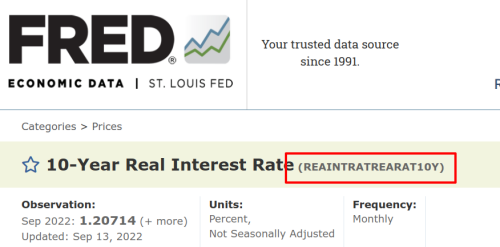
\includegraphics{FRED_series_name.png}
\caption{FRED series name}
\end{figure}

For example, if we want to retrieve the
\href{https://fred.stlouisfed.org/series/REAINTRATREARAT10Y}{10-year
real interest rate}, the corresponding series name is
\texttt{REAINTRATREARAT10Y}. The FRED web page contains additional
useful information such as the time period for which the data is
available, the data frequency (monthly, quarterly, annual) and whether
it's seasonally adjusted.

    To download and plot the 10-year real interest rate, we proceed as
follows:

    \begin{tcolorbox}[breakable, size=fbox, boxrule=1pt, pad at break*=1mm,colback=cellbackground, colframe=cellborder]
\prompt{In}{incolor}{12}{\boxspacing}
\begin{Verbatim}[commandchars=\\\{\}]
\PY{k+kn}{from} \PY{n+nn}{fredapi} \PY{k+kn}{import} \PY{n}{Fred}

\PY{c+c1}{\PYZsh{} Create instance assuming API key is stored as environment variable}
\PY{n}{fred} \PY{o}{=} \PY{n}{Fred}\PY{p}{(}\PY{p}{)}

\PY{c+c1}{\PYZsh{} or specify API key directly}
\PY{c+c1}{\PYZsh{} fred = Fred(api\PYZus{}key=\PYZsq{}INSERT API KEY HERE\PYZsq{})}

\PY{c+c1}{\PYZsh{} Download observations starting from the year 2000 onward}
\PY{n}{series} \PY{o}{=} \PY{n}{fred}\PY{o}{.}\PY{n}{get\PYZus{}series}\PY{p}{(}\PY{l+s+s1}{\PYZsq{}}\PY{l+s+s1}{REAINTRATREARAT10Y}\PY{l+s+s1}{\PYZsq{}}\PY{p}{,} \PY{n}{observation\PYZus{}start}\PY{o}{=}\PY{l+s+s1}{\PYZsq{}}\PY{l+s+s1}{2000\PYZhy{}01\PYZhy{}01}\PY{l+s+s1}{\PYZsq{}}\PY{p}{)}
\end{Verbatim}
\end{tcolorbox}

    \begin{tcolorbox}[breakable, size=fbox, boxrule=1pt, pad at break*=1mm,colback=cellbackground, colframe=cellborder]
\prompt{In}{incolor}{13}{\boxspacing}
\begin{Verbatim}[commandchars=\\\{\}]
\PY{c+c1}{\PYZsh{} Print first 5 observations}
\PY{n}{series}\PY{o}{.}\PY{n}{head}\PY{p}{(}\PY{l+m+mi}{5}\PY{p}{)}
\end{Verbatim}
\end{tcolorbox}

            \begin{tcolorbox}[breakable, size=fbox, boxrule=.5pt, pad at break*=1mm, opacityfill=0]
\prompt{Out}{outcolor}{13}{\boxspacing}
\begin{Verbatim}[commandchars=\\\{\}]
2000-01-01    3.411051
2000-02-01    3.513343
2000-03-01    3.440347
2000-04-01    3.202967
2000-05-01    3.360531
dtype: float64
\end{Verbatim}
\end{tcolorbox}
        
    The data is returned as a pandas \texttt{Series} object with the
corresponding dates set as the index.

    \begin{tcolorbox}[breakable, size=fbox, boxrule=1pt, pad at break*=1mm,colback=cellbackground, colframe=cellborder]
\prompt{In}{incolor}{14}{\boxspacing}
\begin{Verbatim}[commandchars=\\\{\}]
\PY{n}{series}\PY{o}{.}\PY{n}{info}\PY{p}{(}\PY{p}{)}
\end{Verbatim}
\end{tcolorbox}

    \begin{Verbatim}[commandchars=\\\{\}]
<class 'pandas.core.series.Series'>
DatetimeIndex: 273 entries, 2000-01-01 to 2022-09-01
Series name: None
Non-Null Count  Dtype
--------------  -----
273 non-null    float64
dtypes: float64(1)
memory usage: 4.3 KB
    \end{Verbatim}

    \begin{tcolorbox}[breakable, size=fbox, boxrule=1pt, pad at break*=1mm,colback=cellbackground, colframe=cellborder]
\prompt{In}{incolor}{15}{\boxspacing}
\begin{Verbatim}[commandchars=\\\{\}]
\PY{c+c1}{\PYZsh{} Plot interest rate time series}
\PY{n}{series}\PY{o}{.}\PY{n}{plot}\PY{p}{(}\PY{n}{ylabel}\PY{o}{=}\PY{l+s+s1}{\PYZsq{}}\PY{l+s+s1}{10\PYZhy{}year real interest rate}\PY{l+s+s1}{\PYZsq{}}\PY{p}{)}
\end{Verbatim}
\end{tcolorbox}

            \begin{tcolorbox}[breakable, size=fbox, boxrule=.5pt, pad at break*=1mm, opacityfill=0]
\prompt{Out}{outcolor}{15}{\boxspacing}
\begin{Verbatim}[commandchars=\\\{\}]
<AxesSubplot:ylabel='10-year real interest rate'>
\end{Verbatim}
\end{tcolorbox}
        
    \begin{center}
    \adjustimage{max size={0.9\linewidth}{0.9\paperheight}}{unit08_files/unit08_33_1.pdf}
    \end{center}
    
    Other popular time series available on FRED are the
\href{https://fred.stlouisfed.org/series/CPIAUCSL}{CPI},
\href{https://fred.stlouisfed.org/series/GDPC1}{real GDP} and the
\href{https://fred.stlouisfed.org/series/UNRATE}{unemployment rate}.

    \hypertarget{yahoo-finance-data}{%
\subsubsection{Yahoo! Finance data}\label{yahoo-finance-data}}

\href{https://pypi.org/project/yfinance/}{\texttt{yfinance}} is a
user-written library to access data from
\href{https://finance.yahoo.com/}{Yahoo! Finance} using the public API
(see the project's \href{https://github.com/ranaroussi/yfinance}{GitHub
repository} for detailed examples). This project is not affiliated with
Yahoo! Finance and is intended for personal use only. Before using the
library, it needs to be installed from PyPi as follows:

\begin{verbatim}
pip install yfinance 
\end{verbatim}

    \begin{tcolorbox}[breakable, size=fbox, boxrule=1pt, pad at break*=1mm,colback=cellbackground, colframe=cellborder]
\prompt{In}{incolor}{16}{\boxspacing}
\begin{Verbatim}[commandchars=\\\{\}]
\PY{c+c1}{\PYZsh{} When running via Google Colab, uncomment and execute the following line}
\PY{c+c1}{\PYZsh{}! pip install yfinance}
\end{Verbatim}
\end{tcolorbox}

    \texttt{yfinance} allows us to retrieve information for a single symbol
via properties of the \texttt{Ticker} object, or for multiple ticker
symbols at once.

\emph{Example: Retrieving data for a single symbol}

We first use the API to retrieve data for a single symbol, in this case
the \href{https://finance.yahoo.com/quote/\%5EGSPC}{S\&P 500 index}
which has the (somewhat unusual) ticker symbol \texttt{\^{}GSPS}. One
can easily find the desired ticker symbol by searching for some stock,
index, currency or other asset on Yahoo! Finance.

    \begin{tcolorbox}[breakable, size=fbox, boxrule=1pt, pad at break*=1mm,colback=cellbackground, colframe=cellborder]
\prompt{In}{incolor}{17}{\boxspacing}
\begin{Verbatim}[commandchars=\\\{\}]
\PY{k+kn}{import} \PY{n+nn}{yfinance} \PY{k}{as} \PY{n+nn}{yf}

\PY{c+c1}{\PYZsh{} Symbol for S\PYZam{}P 500 index}
\PY{n}{symbol} \PY{o}{=} \PY{l+s+s1}{\PYZsq{}}\PY{l+s+s1}{\PYZca{}GSPC}\PY{l+s+s1}{\PYZsq{}}

\PY{c+c1}{\PYZsh{} Create ticker object}
\PY{n}{ticker} \PY{o}{=} \PY{n}{yf}\PY{o}{.}\PY{n}{Ticker}\PY{p}{(}\PY{n}{symbol}\PY{p}{)}
\end{Verbatim}
\end{tcolorbox}

    We can now use the attributes of the \texttt{ticker} object to get all
sorts of information. For example, we can get some meta data from the
\texttt{info} attribute as follows:

    \begin{tcolorbox}[breakable, size=fbox, boxrule=1pt, pad at break*=1mm,colback=cellbackground, colframe=cellborder]
\prompt{In}{incolor}{18}{\boxspacing}
\begin{Verbatim}[commandchars=\\\{\}]
\PY{c+c1}{\PYZsh{} Descriptive name and asset class}
\PY{n}{shortname} \PY{o}{=} \PY{n}{ticker}\PY{o}{.}\PY{n}{info}\PY{p}{[}\PY{l+s+s1}{\PYZsq{}}\PY{l+s+s1}{shortName}\PY{l+s+s1}{\PYZsq{}}\PY{p}{]}
\PY{n}{quoteType} \PY{o}{=} \PY{n}{ticker}\PY{o}{.}\PY{n}{info}\PY{p}{[}\PY{l+s+s1}{\PYZsq{}}\PY{l+s+s1}{quoteType}\PY{l+s+s1}{\PYZsq{}}\PY{p}{]}

\PY{c+c1}{\PYZsh{} 52\PYZhy{}week low and high}
\PY{n}{low} \PY{o}{=} \PY{n}{ticker}\PY{o}{.}\PY{n}{info}\PY{p}{[}\PY{l+s+s1}{\PYZsq{}}\PY{l+s+s1}{fiftyTwoWeekLow}\PY{l+s+s1}{\PYZsq{}}\PY{p}{]}
\PY{n}{high} \PY{o}{=} \PY{n}{ticker}\PY{o}{.}\PY{n}{info}\PY{p}{[}\PY{l+s+s1}{\PYZsq{}}\PY{l+s+s1}{fiftyTwoWeekHigh}\PY{l+s+s1}{\PYZsq{}}\PY{p}{]}

\PY{n+nb}{print}\PY{p}{(}\PY{l+s+sa}{f}\PY{l+s+s1}{\PYZsq{}}\PY{l+s+si}{\PYZob{}}\PY{n}{shortname}\PY{l+s+si}{\PYZcb{}}\PY{l+s+s1}{ is an }\PY{l+s+si}{\PYZob{}}\PY{n}{quoteType}\PY{l+s+si}{\PYZcb{}}\PY{l+s+s1}{\PYZsq{}}\PY{p}{)}
\PY{n+nb}{print}\PY{p}{(}\PY{l+s+sa}{f}\PY{l+s+s1}{\PYZsq{}}\PY{l+s+si}{\PYZob{}}\PY{n}{shortname}\PY{l+s+si}{\PYZcb{}}\PY{l+s+s1}{ 52\PYZhy{}week range: }\PY{l+s+si}{\PYZob{}}\PY{n}{low}\PY{l+s+si}{\PYZcb{}}\PY{l+s+s1}{ \PYZhy{} }\PY{l+s+si}{\PYZob{}}\PY{n}{high}\PY{l+s+si}{\PYZcb{}}\PY{l+s+s1}{\PYZsq{}}\PY{p}{)}

\PY{c+c1}{\PYZsh{} To see which keys are available, use the keys() method}
\PY{c+c1}{\PYZsh{} ticker.info.keys()}
\end{Verbatim}
\end{tcolorbox}

    \begin{Verbatim}[commandchars=\\\{\}]
S\&P 500 is an INDEX
S\&P 500 52-week range: 3584.13 - 4818.62
    \end{Verbatim}

    We use the \texttt{history} attribute to get detailed price data. Unless
we want all available data, we should select the relevant period using
the \texttt{start=...} and \texttt{end=...} arguments.

    \begin{tcolorbox}[breakable, size=fbox, boxrule=1pt, pad at break*=1mm,colback=cellbackground, colframe=cellborder]
\prompt{In}{incolor}{19}{\boxspacing}
\begin{Verbatim}[commandchars=\\\{\}]
\PY{c+c1}{\PYZsh{} Retrieve daily index values data for this year}
\PY{n}{daily} \PY{o}{=} \PY{n}{ticker}\PY{o}{.}\PY{n}{history}\PY{p}{(}\PY{n}{start}\PY{o}{=}\PY{l+s+s1}{\PYZsq{}}\PY{l+s+s1}{2022\PYZhy{}01\PYZhy{}01}\PY{l+s+s1}{\PYZsq{}}\PY{p}{,} \PY{n}{end}\PY{o}{=}\PY{l+s+s1}{\PYZsq{}}\PY{l+s+s1}{2022\PYZhy{}03\PYZhy{}31}\PY{l+s+s1}{\PYZsq{}}\PY{p}{)}

\PY{c+c1}{\PYZsh{} Print first 5 rows}
\PY{n}{daily}\PY{o}{.}\PY{n}{head}\PY{p}{(}\PY{p}{)}
\end{Verbatim}
\end{tcolorbox}

            \begin{tcolorbox}[breakable, size=fbox, boxrule=.5pt, pad at break*=1mm, opacityfill=0]
\prompt{Out}{outcolor}{19}{\boxspacing}
\begin{Verbatim}[commandchars=\\\{\}]
                   Open         High          Low        Close      Volume  \textbackslash{}
Date
2022-01-03  4778.140137  4796.640137  4758.169922  4796.560059  2775190000
2022-01-04  4804.509766  4818.620117  4774.270020  4793.540039  3641050000
2022-01-05  4787.990234  4797.700195  4699.439941  4700.580078  3733540000
2022-01-06  4693.390137  4725.009766  4671.259766  4696.049805  3371250000
2022-01-07  4697.660156  4707.950195  4662.740234  4677.029785  3279870000

            Dividends  Stock Splits
Date
2022-01-03          0             0
2022-01-04          0             0
2022-01-05          0             0
2022-01-06          0             0
2022-01-07          0             0
\end{Verbatim}
\end{tcolorbox}
        
    We can then use this data to plot the daily closing price and trading
volume.

    \begin{tcolorbox}[breakable, size=fbox, boxrule=1pt, pad at break*=1mm,colback=cellbackground, colframe=cellborder]
\prompt{In}{incolor}{20}{\boxspacing}
\begin{Verbatim}[commandchars=\\\{\}]
\PY{k+kn}{import} \PY{n+nn}{matplotlib}\PY{n+nn}{.}\PY{n+nn}{pyplot} \PY{k}{as} \PY{n+nn}{plt}

\PY{n}{fix}\PY{p}{,} \PY{n}{ax} \PY{o}{=} \PY{n}{plt}\PY{o}{.}\PY{n}{subplots}\PY{p}{(}\PY{l+m+mi}{1}\PY{p}{,} \PY{l+m+mi}{1}\PY{p}{,} \PY{n}{figsize}\PY{o}{=}\PY{p}{(}\PY{l+m+mi}{7}\PY{p}{,}\PY{l+m+mi}{4}\PY{p}{)}\PY{p}{)}

\PY{c+c1}{\PYZsh{} Plot closing price}
\PY{n}{ax}\PY{o}{.}\PY{n}{plot}\PY{p}{(}\PY{n}{daily}\PY{o}{.}\PY{n}{index}\PY{p}{,} \PY{n}{daily}\PY{p}{[}\PY{l+s+s1}{\PYZsq{}}\PY{l+s+s1}{Close}\PY{l+s+s1}{\PYZsq{}}\PY{p}{]}\PY{p}{,} \PY{n}{color}\PY{o}{=}\PY{l+s+s1}{\PYZsq{}}\PY{l+s+s1}{darkblue}\PY{l+s+s1}{\PYZsq{}}\PY{p}{,} \PY{n}{marker}\PY{o}{=}\PY{l+s+s1}{\PYZsq{}}\PY{l+s+s1}{o}\PY{l+s+s1}{\PYZsq{}}\PY{p}{,} \PY{n}{ms}\PY{o}{=}\PY{l+m+mi}{3}\PY{p}{,} \PY{n}{lw}\PY{o}{=}\PY{l+m+mi}{1}\PY{p}{)}

\PY{c+c1}{\PYZsh{} Create secondary y\PYZhy{}axis for trading volume}
\PY{n}{ax2} \PY{o}{=} \PY{n}{ax}\PY{o}{.}\PY{n}{twinx}\PY{p}{(}\PY{p}{)}

\PY{c+c1}{\PYZsh{} Plot trading volume as bar chart}
\PY{n}{ax2}\PY{o}{.}\PY{n}{bar}\PY{p}{(}\PY{n}{daily}\PY{o}{.}\PY{n}{index}\PY{p}{,} \PY{n}{daily}\PY{p}{[}\PY{l+s+s1}{\PYZsq{}}\PY{l+s+s1}{Volume}\PY{l+s+s1}{\PYZsq{}}\PY{p}{]}\PY{p}{,} \PY{n}{color}\PY{o}{=}\PY{l+s+s1}{\PYZsq{}}\PY{l+s+s1}{\PYZsh{}666666}\PY{l+s+s1}{\PYZsq{}}\PY{p}{,} \PY{n}{alpha}\PY{o}{=}\PY{l+m+mf}{0.4}\PY{p}{,} \PY{n}{zorder}\PY{o}{=}\PY{o}{\PYZhy{}}\PY{l+m+mi}{1}\PY{p}{,} \PY{n}{lw}\PY{o}{=}\PY{l+m+mi}{0}\PY{p}{)}
\PY{n}{ax2}\PY{o}{.}\PY{n}{set\PYZus{}ylim}\PY{p}{(}\PY{p}{(}\PY{l+m+mf}{0.0}\PY{p}{,} \PY{l+m+mf}{1.0e10}\PY{p}{)}\PY{p}{)}
\end{Verbatim}
\end{tcolorbox}

            \begin{tcolorbox}[breakable, size=fbox, boxrule=.5pt, pad at break*=1mm, opacityfill=0]
\prompt{Out}{outcolor}{20}{\boxspacing}
\begin{Verbatim}[commandchars=\\\{\}]
(0.0, 10000000000.0)
\end{Verbatim}
\end{tcolorbox}
        
    \begin{center}
    \adjustimage{max size={0.9\linewidth}{0.9\paperheight}}{unit08_files/unit08_44_1.pdf}
    \end{center}
    
    \emph{Example: Retrieving data for multiple symbols}

We can download trading data for multiple symbols at once using the
\texttt{download()} function. Unlike the \texttt{Ticker} class, this
immediately returns a \texttt{DataFrame} containing data similar to the
\texttt{history} method we called previosuly, but now the column index
contains an additional level for each ticker symbol. For example, to get
the trading data for Amazon and Microsoft for the last 3 months, we
proceed as follows:

    \begin{tcolorbox}[breakable, size=fbox, boxrule=1pt, pad at break*=1mm,colback=cellbackground, colframe=cellborder]
\prompt{In}{incolor}{21}{\boxspacing}
\begin{Verbatim}[commandchars=\\\{\}]
\PY{k+kn}{import} \PY{n+nn}{yfinance} \PY{k}{as} \PY{n+nn}{yf}

\PY{c+c1}{\PYZsh{} Get data for Amazon (AMZN) and Microsoft (MSFT) for the last three months.}
\PY{c+c1}{\PYZsh{} valid intervals for the \PYZsq{}period\PYZsq{} argument are: }
\PY{c+c1}{\PYZsh{}   1m,2m,5m,15m,30m,60m,90m,1h,1d,5d,1wk,1mo,3mo}
\PY{n}{data} \PY{o}{=} \PY{n}{yf}\PY{o}{.}\PY{n}{download}\PY{p}{(}\PY{l+s+s2}{\PYZdq{}}\PY{l+s+s2}{AMZN MSFT}\PY{l+s+s2}{\PYZdq{}}\PY{p}{,} \PY{n}{period}\PY{o}{=}\PY{l+s+s1}{\PYZsq{}}\PY{l+s+s1}{3mo}\PY{l+s+s1}{\PYZsq{}}\PY{p}{)}
\PY{n}{data}\PY{o}{.}\PY{n}{head}\PY{p}{(}\PY{p}{)}
\end{Verbatim}
\end{tcolorbox}

    \begin{Verbatim}[commandchars=\\\{\}]
[*********************100\%***********************]  2 of 2 completed
    \end{Verbatim}

            \begin{tcolorbox}[breakable, size=fbox, boxrule=.5pt, pad at break*=1mm, opacityfill=0]
\prompt{Out}{outcolor}{21}{\boxspacing}
\begin{Verbatim}[commandchars=\\\{\}]
             Adj Close                   Close                    High  \textbackslash{}
                  AMZN        MSFT        AMZN        MSFT        AMZN
Date
2022-07-05  113.500000  262.293274  113.500000  262.850006  114.080002
2022-07-06  114.330002  265.646118  114.330002  266.209991  115.480003
2022-07-07  116.330002  267.831482  116.330002  268.399994  116.989998
2022-07-08  115.540001  267.093079  115.540001  267.660004  116.580002
2022-07-11  111.750000  263.949738  111.750000  264.510010  114.300003

                               Low                    Open              \textbackslash{}
                  MSFT        AMZN        MSFT        AMZN        MSFT
Date
2022-07-05  262.980011  106.320000  254.740005  107.599998  256.160004
2022-07-06  267.989990  112.010002  262.399994  113.209999  263.750000
2022-07-07  269.059998  113.489998  265.019989  113.849998  265.119995
2022-07-08  268.100006  113.690002  263.290009  114.599998  264.790009
2022-07-11  266.529999  110.870003  262.179993  114.080002  265.649994

              Volume
                AMZN      MSFT
Date
2022-07-05  76583700  22941000
2022-07-06  66958900  23824400
2022-07-07  57872300  20859900
2022-07-08  45719700  19658800
2022-07-11  53487600  19455200
\end{Verbatim}
\end{tcolorbox}
        
    To extract data for a particular symbol, we have to take into account
the hierarchical column index:

    \begin{tcolorbox}[breakable, size=fbox, boxrule=1pt, pad at break*=1mm,colback=cellbackground, colframe=cellborder]
\prompt{In}{incolor}{22}{\boxspacing}
\begin{Verbatim}[commandchars=\\\{\}]
\PY{c+c1}{\PYZsh{} Use hierarchical indexing to get data for Amazon}
\PY{n}{data}\PY{p}{[}\PY{p}{(}\PY{l+s+s1}{\PYZsq{}}\PY{l+s+s1}{Close}\PY{l+s+s1}{\PYZsq{}}\PY{p}{,} \PY{l+s+s1}{\PYZsq{}}\PY{l+s+s1}{AMZN}\PY{l+s+s1}{\PYZsq{}}\PY{p}{)}\PY{p}{]}\PY{o}{.}\PY{n}{head}\PY{p}{(}\PY{p}{)}
\end{Verbatim}
\end{tcolorbox}

            \begin{tcolorbox}[breakable, size=fbox, boxrule=.5pt, pad at break*=1mm, opacityfill=0]
\prompt{Out}{outcolor}{22}{\boxspacing}
\begin{Verbatim}[commandchars=\\\{\}]
Date
2022-07-05    113.500000
2022-07-06    114.330002
2022-07-07    116.330002
2022-07-08    115.540001
2022-07-11    111.750000
Name: (Close, AMZN), dtype: float64
\end{Verbatim}
\end{tcolorbox}
        
    \begin{tcolorbox}[breakable, size=fbox, boxrule=1pt, pad at break*=1mm,colback=cellbackground, colframe=cellborder]
\prompt{In}{incolor}{23}{\boxspacing}
\begin{Verbatim}[commandchars=\\\{\}]
\PY{c+c1}{\PYZsh{} Plot daily returns for both stocks}
\PY{n}{returns} \PY{o}{=} \PY{n}{data}\PY{p}{[}\PY{l+s+s1}{\PYZsq{}}\PY{l+s+s1}{Close}\PY{l+s+s1}{\PYZsq{}}\PY{p}{]}\PY{o}{.}\PY{n}{diff}\PY{p}{(}\PY{p}{)} \PY{o}{/} \PY{n}{data}\PY{p}{[}\PY{l+s+s1}{\PYZsq{}}\PY{l+s+s1}{Close}\PY{l+s+s1}{\PYZsq{}}\PY{p}{]}
\PY{n}{returns}\PY{o}{.}\PY{n}{plot}\PY{p}{(}\PY{n}{y}\PY{o}{=}\PY{p}{[}\PY{l+s+s1}{\PYZsq{}}\PY{l+s+s1}{AMZN}\PY{l+s+s1}{\PYZsq{}}\PY{p}{,} \PY{l+s+s1}{\PYZsq{}}\PY{l+s+s1}{MSFT}\PY{l+s+s1}{\PYZsq{}}\PY{p}{]}\PY{p}{)}
\end{Verbatim}
\end{tcolorbox}

            \begin{tcolorbox}[breakable, size=fbox, boxrule=.5pt, pad at break*=1mm, opacityfill=0]
\prompt{Out}{outcolor}{23}{\boxspacing}
\begin{Verbatim}[commandchars=\\\{\}]
<AxesSubplot:xlabel='Date'>
\end{Verbatim}
\end{tcolorbox}
        
    \begin{center}
    \adjustimage{max size={0.9\linewidth}{0.9\paperheight}}{unit08_files/unit08_49_1.pdf}
    \end{center}
    
    \hypertarget{nasdaq-data-api-formerly-quandl}{%
\subsubsection{NASDAQ data API (formerly
quandl)}\label{nasdaq-data-api-formerly-quandl}}

The NASDAQ stock exchange provides an open-source Python library hosted
on \href{https://github.com/Nasdaq/data-link-python}{GitHub} to access
various types of financial data (not only those traded on NASDAQ), see
\href{https://data.nasdaq.com/}{here} for details. The detailed API
documentation can be found at
\href{https://docs.data.nasdaq.com/docs}{here}. This data API was
formerly known as \href{https://github.com/quandl/quandl-python}{quandl}
which is no longer actively maintained but might still work.

Before using this service, you need to make sure that the Python package
is installed. Depending on how you launched this notebook, you may need
to execute the following code to install \texttt{nasdaq-data-link}:

\begin{verbatim}
pip install nasdaq-data-link
\end{verbatim}

Various types of data are available via this service and can be found
using the online search at \url{https://data.nasdaq.com/search}.

\begin{itemize}
\item
  Data come from various data provides. To select a data set, you
  usually have to specify a string of the form
  \texttt{\textquotesingle{}PROVIDER/SERIES\textquotesingle{}} where
  \texttt{\textquotesingle{}PROVIDER\textquotesingle{}} is the name of
  the provider (\eg \texttt{\textquotesingle{}FRED\textquotesingle{}}
  or \texttt{\textquotesingle{}BOE\textquotesingle{}}) and
  \texttt{\textquotesingle{}SERIES\textquotesingle{}} is the name of the
  time series.
\item
  Most of these data require a subscription or at least a free NASDAQ
  account. Once you have an account, you will need to get an API key and
  specify it when retrieving data. See the above links for details.
\item
  Some commercial data series include sample data that can be used
  without a subscription but requires a free NASDAQ account.
\item
  Some data series are freely available without a subscription or an
  account. These are often taken from other freely available data sets
  such as \href{https://fred.stlouisfed.org/}{FRED} or
  \href{https://www.blockchain.com/}{blockchain.com}. We'll be using
  these to demonstrate how the API works.

  \emph{Important:} Even for freely available data, NASDAQ imposes a cap
  of 50 calls per day. You need to register to get around this.
\end{itemize}

The data is returned as pandas \texttt{DataFrame} object (or
alternatively as an NumPy array).

    \begin{tcolorbox}[breakable, size=fbox, boxrule=1pt, pad at break*=1mm,colback=cellbackground, colframe=cellborder]
\prompt{In}{incolor}{24}{\boxspacing}
\begin{Verbatim}[commandchars=\\\{\}]
\PY{c+c1}{\PYZsh{} When running via Google Colab, uncomment and execute the following line}
\PY{c+c1}{\PYZsh{}! pip install nasdaq\PYZhy{}data\PYZhy{}link}
\end{Verbatim}
\end{tcolorbox}

    \emph{Example: Data from the Bank of England}

Let's start by retrieving some macroeconomic times series from the Bank
of England (BOE). It's not always straightforward to find the name of
the time series one is looking for, but you can see some of the
available time series
\href{https://data.nasdaq.com/data/BOE-bank-of-england-official-statistics/documentation}{here}.
The name will vary depending on the type of data (interest rate,
exchange rate), the frequency and how it is aggregated (daily, last day
of the month, monthly average) and a currency pair, if applicable.

    \begin{tcolorbox}[breakable, size=fbox, boxrule=1pt, pad at break*=1mm,colback=cellbackground, colframe=cellborder]
\prompt{In}{incolor}{25}{\boxspacing}
\begin{Verbatim}[commandchars=\\\{\}]
\PY{c+c1}{\PYZsh{} Retrieve 5\PYZhy{}year real implied yield on UK government bonds}
\PY{k+kn}{import} \PY{n+nn}{nasdaqdatalink} \PY{k}{as} \PY{n+nn}{ndl}
\PY{n}{df} \PY{o}{=} \PY{n}{ndl}\PY{o}{.}\PY{n}{get}\PY{p}{(}\PY{l+s+s1}{\PYZsq{}}\PY{l+s+s1}{BOE/IUMASRIF}\PY{l+s+s1}{\PYZsq{}}\PY{p}{)}

\PY{c+c1}{\PYZsh{} Rename column which is always called \PYZsq{}Value\PYZsq{}}
\PY{n}{df} \PY{o}{=} \PY{n}{df}\PY{o}{.}\PY{n}{rename}\PY{p}{(}\PY{n}{columns}\PY{o}{=}\PY{p}{\PYZob{}}\PY{l+s+s1}{\PYZsq{}}\PY{l+s+s1}{Value}\PY{l+s+s1}{\PYZsq{}}\PY{p}{:} \PY{l+s+s1}{\PYZsq{}}\PY{l+s+s1}{Yield}\PY{l+s+s1}{\PYZsq{}}\PY{p}{\PYZcb{}}\PY{p}{)}

\PY{c+c1}{\PYZsh{} Plot time series }
\PY{n}{df}\PY{o}{.}\PY{n}{plot}\PY{p}{(}\PY{n}{ylabel}\PY{o}{=}\PY{l+s+s1}{\PYZsq{}}\PY{l+s+s1}{5 Year Real Implied Forward (Monthly)}\PY{l+s+s1}{\PYZsq{}}\PY{p}{)}
\end{Verbatim}
\end{tcolorbox}

            \begin{tcolorbox}[breakable, size=fbox, boxrule=.5pt, pad at break*=1mm, opacityfill=0]
\prompt{Out}{outcolor}{25}{\boxspacing}
\begin{Verbatim}[commandchars=\\\{\}]
<AxesSubplot:xlabel='Date', ylabel='5 Year Real Implied Forward (Monthly)'>
\end{Verbatim}
\end{tcolorbox}
        
    \begin{center}
    \adjustimage{max size={0.9\linewidth}{0.9\paperheight}}{unit08_files/unit08_53_1.pdf}
    \end{center}
    
    As another example, we retrieve the US dollar / Sterling exchange rate
at a monthly frequency (this is determined by the name of the time
series used where \texttt{ML} requests the monthly series, using the
last observation for each month). Note that we can pass additional
arguments, for example restricting the time period we want to retrieve
using \texttt{start\_date} and \texttt{end\_date}.

    \begin{tcolorbox}[breakable, size=fbox, boxrule=1pt, pad at break*=1mm,colback=cellbackground, colframe=cellborder]
\prompt{In}{incolor}{26}{\boxspacing}
\begin{Verbatim}[commandchars=\\\{\}]
\PY{c+c1}{\PYZsh{} Get USD / GDP exchange rate using the last observation for each month.}
\PY{n}{df} \PY{o}{=} \PY{n}{ndl}\PY{o}{.}\PY{n}{get}\PY{p}{(}\PY{l+s+s1}{\PYZsq{}}\PY{l+s+s1}{BOE/XUMLUSS}\PY{l+s+s1}{\PYZsq{}}\PY{p}{,} \PY{n}{start\PYZus{}date}\PY{o}{=}\PY{l+s+s1}{\PYZsq{}}\PY{l+s+s1}{2000\PYZhy{}01\PYZhy{}31}\PY{l+s+s1}{\PYZsq{}}\PY{p}{)}
\PY{n}{df} \PY{o}{=} \PY{n}{df}\PY{o}{.}\PY{n}{rename}\PY{p}{(}\PY{n}{columns}\PY{o}{=}\PY{p}{\PYZob{}}\PY{l+s+s1}{\PYZsq{}}\PY{l+s+s1}{Value}\PY{l+s+s1}{\PYZsq{}}\PY{p}{:} \PY{l+s+s1}{\PYZsq{}}\PY{l+s+s1}{USD\PYZus{}GBP}\PY{l+s+s1}{\PYZsq{}}\PY{p}{\PYZcb{}}\PY{p}{)}

\PY{c+c1}{\PYZsh{} Plot USD/GBP time series}
\PY{n}{df}\PY{o}{.}\PY{n}{plot}\PY{p}{(}\PY{n}{ylabel}\PY{o}{=}\PY{l+s+s1}{\PYZsq{}}\PY{l+s+s1}{USD/GBP exchange rate}\PY{l+s+s1}{\PYZsq{}}\PY{p}{)}
\end{Verbatim}
\end{tcolorbox}

            \begin{tcolorbox}[breakable, size=fbox, boxrule=.5pt, pad at break*=1mm, opacityfill=0]
\prompt{Out}{outcolor}{26}{\boxspacing}
\begin{Verbatim}[commandchars=\\\{\}]
<AxesSubplot:xlabel='Date', ylabel='USD/GBP exchange rate'>
\end{Verbatim}
\end{tcolorbox}
        
    \begin{center}
    \adjustimage{max size={0.9\linewidth}{0.9\paperheight}}{unit08_files/unit08_55_1.pdf}
    \end{center}
    
    \emph{Example: Data from blockchain.com}

The NASDAQ data link also supports retrieving data on cryptocurrencies.
For example, there is a freely accessible time series for the price of
Bitcoin in USD.

    \begin{tcolorbox}[breakable, size=fbox, boxrule=1pt, pad at break*=1mm,colback=cellbackground, colframe=cellborder]
\prompt{In}{incolor}{27}{\boxspacing}
\begin{Verbatim}[commandchars=\\\{\}]
\PY{k+kn}{import} \PY{n+nn}{nasdaqdatalink} \PY{k}{as} \PY{n+nn}{ndl}

\PY{c+c1}{\PYZsh{} Retrieve price of BTC in USD for 2022}
\PY{n}{df} \PY{o}{=} \PY{n}{ndl}\PY{o}{.}\PY{n}{get}\PY{p}{(}\PY{l+s+s1}{\PYZsq{}}\PY{l+s+s1}{BCHAIN/MKPRU}\PY{l+s+s1}{\PYZsq{}}\PY{p}{,} \PY{n}{start\PYZus{}date}\PY{o}{=}\PY{l+s+s1}{\PYZsq{}}\PY{l+s+s1}{2022\PYZhy{}01\PYZhy{}31}\PY{l+s+s1}{\PYZsq{}}\PY{p}{)}

\PY{c+c1}{\PYZsh{} Change column name to something more descriptive}
\PY{n}{df} \PY{o}{=} \PY{n}{df}\PY{o}{.}\PY{n}{rename}\PY{p}{(}\PY{n}{columns}\PY{o}{=}\PY{p}{\PYZob{}}\PY{l+s+s1}{\PYZsq{}}\PY{l+s+s1}{Value}\PY{l+s+s1}{\PYZsq{}}\PY{p}{:} \PY{l+s+s1}{\PYZsq{}}\PY{l+s+s1}{BTC\PYZus{}USD}\PY{l+s+s1}{\PYZsq{}}\PY{p}{\PYZcb{}}\PY{p}{)}

\PY{c+c1}{\PYZsh{} Plot time series}
\PY{n}{df}\PY{o}{.}\PY{n}{plot}\PY{p}{(}\PY{n}{ylabel}\PY{o}{=}\PY{l+s+s1}{\PYZsq{}}\PY{l+s+s1}{BTC price in USD}\PY{l+s+s1}{\PYZsq{}}\PY{p}{)}
\end{Verbatim}
\end{tcolorbox}

            \begin{tcolorbox}[breakable, size=fbox, boxrule=.5pt, pad at break*=1mm, opacityfill=0]
\prompt{Out}{outcolor}{27}{\boxspacing}
\begin{Verbatim}[commandchars=\\\{\}]
<AxesSubplot:xlabel='Date', ylabel='BTC price in USD'>
\end{Verbatim}
\end{tcolorbox}
        
    \begin{center}
    \adjustimage{max size={0.9\linewidth}{0.9\paperheight}}{unit08_files/unit08_57_1.pdf}
    \end{center}
    
    \emph{Example: Historical stock data}

As a final example, we obtain the trading data for the stock of Apple
(ticker symbol \texttt{AAPL}) for the year 2001. Such data is often not
available without a subscription or a login, but it works if the
requested time period is sufficiently far in the past!

    \begin{tcolorbox}[breakable, size=fbox, boxrule=1pt, pad at break*=1mm,colback=cellbackground, colframe=cellborder]
\prompt{In}{incolor}{28}{\boxspacing}
\begin{Verbatim}[commandchars=\\\{\}]
\PY{c+c1}{\PYZsh{} Retrieve stock data for Apple (ticker symbol AAPL)}
\PY{n}{df} \PY{o}{=} \PY{n}{ndl}\PY{o}{.}\PY{n}{get}\PY{p}{(}\PY{l+s+s2}{\PYZdq{}}\PY{l+s+s2}{WIKI/AAPL}\PY{l+s+s2}{\PYZdq{}}\PY{p}{,} \PY{n}{start\PYZus{}date}\PY{o}{=}\PY{l+s+s1}{\PYZsq{}}\PY{l+s+s1}{2000\PYZhy{}01\PYZhy{}01}\PY{l+s+s1}{\PYZsq{}}\PY{p}{,} \PY{n}{end\PYZus{}date}\PY{o}{=}\PY{l+s+s1}{\PYZsq{}}\PY{l+s+s1}{2000\PYZhy{}12\PYZhy{}31}\PY{l+s+s1}{\PYZsq{}}\PY{p}{)}
\end{Verbatim}
\end{tcolorbox}

    Unlike in the previous examples, this data contains not only a single
value, but a whole range of variables including the opening and closing
price, the trading volume, \etc:

    \begin{tcolorbox}[breakable, size=fbox, boxrule=1pt, pad at break*=1mm,colback=cellbackground, colframe=cellborder]
\prompt{In}{incolor}{29}{\boxspacing}
\begin{Verbatim}[commandchars=\\\{\}]
\PY{n}{df}\PY{o}{.}\PY{n}{info}\PY{p}{(}\PY{p}{)}
\end{Verbatim}
\end{tcolorbox}

    \begin{Verbatim}[commandchars=\\\{\}]
<class 'pandas.core.frame.DataFrame'>
DatetimeIndex: 252 entries, 2000-01-03 to 2000-12-29
Data columns (total 12 columns):
 \#   Column       Non-Null Count  Dtype
---  ------       --------------  -----
 0   Open         252 non-null    float64
 1   High         252 non-null    float64
 2   Low          252 non-null    float64
 3   Close        252 non-null    float64
 4   Volume       252 non-null    float64
 5   Ex-Dividend  252 non-null    float64
 6   Split Ratio  252 non-null    float64
 7   Adj. Open    252 non-null    float64
 8   Adj. High    252 non-null    float64
 9   Adj. Low     252 non-null    float64
 10  Adj. Close   252 non-null    float64
 11  Adj. Volume  252 non-null    float64
dtypes: float64(12)
memory usage: 25.6 KB
    \end{Verbatim}

    To plot a specific column, we can use the \texttt{y=...} argument to
\texttt{DataFrame.plot()}.

    \begin{tcolorbox}[breakable, size=fbox, boxrule=1pt, pad at break*=1mm,colback=cellbackground, colframe=cellborder]
\prompt{In}{incolor}{30}{\boxspacing}
\begin{Verbatim}[commandchars=\\\{\}]
\PY{n}{df}\PY{o}{.}\PY{n}{plot}\PY{p}{(}\PY{n}{y}\PY{o}{=}\PY{l+s+s1}{\PYZsq{}}\PY{l+s+s1}{Close}\PY{l+s+s1}{\PYZsq{}}\PY{p}{,} \PY{n}{ylabel}\PY{o}{=}\PY{l+s+s1}{\PYZsq{}}\PY{l+s+s1}{Stock prive of AAPL}\PY{l+s+s1}{\PYZsq{}}\PY{p}{)}
\end{Verbatim}
\end{tcolorbox}

            \begin{tcolorbox}[breakable, size=fbox, boxrule=.5pt, pad at break*=1mm, opacityfill=0]
\prompt{Out}{outcolor}{30}{\boxspacing}
\begin{Verbatim}[commandchars=\\\{\}]
<AxesSubplot:xlabel='Date', ylabel='Stock prive of AAPL'>
\end{Verbatim}
\end{tcolorbox}
        
    \begin{center}
    \adjustimage{max size={0.9\linewidth}{0.9\paperheight}}{unit08_files/unit08_63_1.pdf}
    \end{center}
    
    \hypertarget{pandas-datareader}{%
\subsubsection{Pandas Datareader}\label{pandas-datareader}}

\href{https://github.com/pydata/pandas-datareader}{\texttt{pandas-datareader}}
is a Python library that fetches online data from multiple sources and
returns them as pandas \texttt{DataFrame} objects. Despite its name,
this library is not included in \texttt{pandas} and may need to be
installed separately, \eg by running

\begin{verbatim}
pip install pandas-datareader
\end{verbatim}

The aim is to provide a uniform API to access data from multiple
sources, including those we covered earlier. See the official
\href{https://pandas-datareader.readthedocs.io/en/latest/}{documentation}
for supported data sources and how to access them.

    \begin{tcolorbox}[breakable, size=fbox, boxrule=1pt, pad at break*=1mm,colback=cellbackground, colframe=cellborder]
\prompt{In}{incolor}{31}{\boxspacing}
\begin{Verbatim}[commandchars=\\\{\}]
\PY{c+c1}{\PYZsh{} Uncomment and execute the following line if running in Google Colab}
\PY{c+c1}{\PYZsh{} ! pip install pandas\PYZhy{}datareader}
\end{Verbatim}
\end{tcolorbox}

    \emph{Example: Downloading data from FRED}

As a first illustration, we fetch macroeconomic data from
\href{https://fred.stlouisfed.org/}{FRED}, but instead of
\texttt{fredapi} we use \texttt{pandas-datareader} and set the data
source to \texttt{\textquotesingle{}fred\textquotesingle{}}. No API key
is required for this particular data source, but this is not true for
all data sources supported by \texttt{pandas-datareader}.

Note that we find the name of the series we want to download in the same
way as previously discussed in the section on FRED.

    \begin{tcolorbox}[breakable, size=fbox, boxrule=1pt, pad at break*=1mm,colback=cellbackground, colframe=cellborder]
\prompt{In}{incolor}{32}{\boxspacing}
\begin{Verbatim}[commandchars=\\\{\}]
\PY{c+c1}{\PYZsh{} The convention is to import this library as web}
\PY{k+kn}{import} \PY{n+nn}{pandas\PYZus{}datareader}\PY{n+nn}{.}\PY{n+nn}{data} \PY{k}{as} \PY{n+nn}{web}

\PY{c+c1}{\PYZsh{} define start and end dates}
\PY{n}{start\PYZus{}date} \PY{o}{=} \PY{l+s+s2}{\PYZdq{}}\PY{l+s+s2}{2000\PYZhy{}01\PYZhy{}01}\PY{l+s+s2}{\PYZdq{}}
\PY{n}{end\PYZus{}date} \PY{o}{=} \PY{l+s+s2}{\PYZdq{}}\PY{l+s+s2}{2021\PYZhy{}12\PYZhy{}31}\PY{l+s+s2}{\PYZdq{}}

\PY{c+c1}{\PYZsh{} Specify series name as first and \PYZsq{}fred\PYZsq{} data source as second argument}
\PY{n}{gdp} \PY{o}{=} \PY{n}{web}\PY{o}{.}\PY{n}{DataReader}\PY{p}{(}\PY{l+s+s1}{\PYZsq{}}\PY{l+s+s1}{GDP}\PY{l+s+s1}{\PYZsq{}}\PY{p}{,} \PY{l+s+s1}{\PYZsq{}}\PY{l+s+s1}{fred}\PY{l+s+s1}{\PYZsq{}}\PY{p}{,} \PY{n}{start\PYZus{}date}\PY{p}{,} \PY{n}{end\PYZus{}date}\PY{p}{)}

\PY{c+c1}{\PYZsh{} Show first 3 observations}
\PY{n}{gdp}\PY{o}{.}\PY{n}{head}\PY{p}{(}\PY{l+m+mi}{3}\PY{p}{)}
\end{Verbatim}
\end{tcolorbox}

            \begin{tcolorbox}[breakable, size=fbox, boxrule=.5pt, pad at break*=1mm, opacityfill=0]
\prompt{Out}{outcolor}{32}{\boxspacing}
\begin{Verbatim}[commandchars=\\\{\}]
                  GDP
DATE
2000-01-01  10002.179
2000-04-01  10247.720
2000-07-01  10318.165
\end{Verbatim}
\end{tcolorbox}
        
    We can also fetch multiple series at the same time, for example the CPI
and the unemployment rate.

    \begin{tcolorbox}[breakable, size=fbox, boxrule=1pt, pad at break*=1mm,colback=cellbackground, colframe=cellborder]
\prompt{In}{incolor}{33}{\boxspacing}
\begin{Verbatim}[commandchars=\\\{\}]
\PY{n}{data} \PY{o}{=} \PY{n}{web}\PY{o}{.}\PY{n}{DataReader}\PY{p}{(}\PY{p}{[}\PY{l+s+s1}{\PYZsq{}}\PY{l+s+s1}{CPIAUCSL}\PY{l+s+s1}{\PYZsq{}}\PY{p}{,} \PY{l+s+s1}{\PYZsq{}}\PY{l+s+s1}{UNRATE}\PY{l+s+s1}{\PYZsq{}}\PY{p}{]}\PY{p}{,} \PY{n}{data\PYZus{}source}\PY{o}{=}\PY{l+s+s1}{\PYZsq{}}\PY{l+s+s1}{fred}\PY{l+s+s1}{\PYZsq{}}\PY{p}{,} \PY{n}{start}\PY{o}{=}\PY{l+s+s1}{\PYZsq{}}\PY{l+s+s1}{2020\PYZhy{}01\PYZhy{}01}\PY{l+s+s1}{\PYZsq{}}\PY{p}{)}
\PY{n}{data}\PY{o}{.}\PY{n}{head}\PY{p}{(}\PY{l+m+mi}{3}\PY{p}{)}
\end{Verbatim}
\end{tcolorbox}

            \begin{tcolorbox}[breakable, size=fbox, boxrule=.5pt, pad at break*=1mm, opacityfill=0]
\prompt{Out}{outcolor}{33}{\boxspacing}
\begin{Verbatim}[commandchars=\\\{\}]
            CPIAUCSL  UNRATE
DATE
2020-01-01   258.682     3.5
2020-02-01   259.007     3.5
2020-03-01   258.165     4.4
\end{Verbatim}
\end{tcolorbox}
        
    \emph{Example: Download data from Yahoo! Finance}

As another example, we can use \texttt{pandas-datareader} as a client
for Yahoo! Finance by specifying
\texttt{\textquotesingle{}yahoo\textquotesingle{}} as the data source.
As with \texttt{yfinance} we discussed earlier, we use the search
function on \href{https://finance.yahoo.com}{Yahoo! Finance} to identify
the ticker symbol for the data series we are interested in.

The example below also illustrates that we can optionally use instances
of \texttt{datetime} to define the sample period instead of plain
strings.

    \begin{tcolorbox}[breakable, size=fbox, boxrule=1pt, pad at break*=1mm,colback=cellbackground, colframe=cellborder]
\prompt{In}{incolor}{34}{\boxspacing}
\begin{Verbatim}[commandchars=\\\{\}]
\PY{k+kn}{import} \PY{n+nn}{pandas\PYZus{}datareader}\PY{n+nn}{.}\PY{n+nn}{data} \PY{k}{as} \PY{n+nn}{web}
\PY{k+kn}{import} \PY{n+nn}{datetime}

\PY{c+c1}{\PYZsh{} Instead of strings, we can define period in terms of datetime objects:}
\PY{c+c1}{\PYZsh{} Sample period: 2011\PYZhy{}01\PYZhy{}1 to 2021\PYZhy{}12\PYZhy{}31}
\PY{n}{start} \PY{o}{=} \PY{n}{datetime}\PY{o}{.}\PY{n}{datetime}\PY{p}{(}\PY{l+m+mi}{2011}\PY{p}{,} \PY{l+m+mi}{1}\PY{p}{,} \PY{l+m+mi}{1}\PY{p}{)}
\PY{n}{end} \PY{o}{=} \PY{n}{datetime}\PY{o}{.}\PY{n}{datetime}\PY{p}{(}\PY{l+m+mi}{2021}\PY{p}{,} \PY{l+m+mi}{12}\PY{p}{,} \PY{l+m+mi}{31}\PY{p}{)}

\PY{c+c1}{\PYZsh{} Fetch stock price data for Tesla (ticker symbol TSLA)}
\PY{n}{data} \PY{o}{=} \PY{n}{web}\PY{o}{.}\PY{n}{DataReader}\PY{p}{(}\PY{l+s+s1}{\PYZsq{}}\PY{l+s+s1}{TSLA}\PY{l+s+s1}{\PYZsq{}}\PY{p}{,} \PY{n}{data\PYZus{}source}\PY{o}{=}\PY{l+s+s1}{\PYZsq{}}\PY{l+s+s1}{yahoo}\PY{l+s+s1}{\PYZsq{}}\PY{p}{,} \PY{n}{start}\PY{o}{=}\PY{n}{start}\PY{p}{,} \PY{n}{end}\PY{o}{=}\PY{n}{end}\PY{p}{)}

\PY{n}{data}\PY{o}{.}\PY{n}{head}\PY{p}{(}\PY{l+m+mi}{3}\PY{p}{)}
\end{Verbatim}
\end{tcolorbox}

            \begin{tcolorbox}[breakable, size=fbox, boxrule=.5pt, pad at break*=1mm, opacityfill=0]
\prompt{Out}{outcolor}{34}{\boxspacing}
\begin{Verbatim}[commandchars=\\\{\}]
                High       Low      Open     Close      Volume  Adj Close
Date
2011-01-03  1.800000  1.726667  1.789333  1.774667  19245000.0   1.774667
2011-01-04  1.796667  1.734667  1.777333  1.778000  17811000.0   1.778000
2011-01-05  1.793333  1.746000  1.765333  1.788667  21700500.0   1.788667
\end{Verbatim}
\end{tcolorbox}
        

\hypertarget{pickling}{%
\subsection{Pickling}\label{pickling}}

A wholly different approach to data I/O is taken by Python's built-in
\href{https://docs.python.org/3/library/pickle.html}{\texttt{pickle}}
module. Almost any Python object can be dumped into a binary file and
read back using \texttt{pickle.dump()} and \texttt{pickle.load()}.

The big advantage over other methods is that hierarchies of objects are
automatically supported. For example, we can pickle a list containing a
\texttt{tuple}, a string and a NumPy array:

    \begin{tcolorbox}[breakable, size=fbox, boxrule=1pt, pad at break*=1mm,colback=cellbackground, colframe=cellborder]
\prompt{In}{incolor}{35}{\boxspacing}
\begin{Verbatim}[commandchars=\\\{\}]
\PY{k+kn}{import} \PY{n+nn}{numpy} \PY{k}{as} \PY{n+nn}{np}
\PY{k+kn}{import} \PY{n+nn}{pickle}
\PY{k+kn}{import} \PY{n+nn}{tempfile}
\PY{k+kn}{import} \PY{n+nn}{os}\PY{n+nn}{.}\PY{n+nn}{path}

\PY{c+c1}{\PYZsh{} Generate 2d array of integers}
\PY{n}{arr} \PY{o}{=} \PY{n}{np}\PY{o}{.}\PY{n}{arange}\PY{p}{(}\PY{l+m+mi}{10}\PY{p}{)}\PY{o}{.}\PY{n}{reshape}\PY{p}{(}\PY{p}{(}\PY{l+m+mi}{2}\PY{p}{,} \PY{o}{\PYZhy{}}\PY{l+m+mi}{1}\PY{p}{)}\PY{p}{)}
\PY{n}{tpl} \PY{o}{=} \PY{p}{(}\PY{l+m+mi}{1}\PY{p}{,} \PY{l+m+mi}{2}\PY{p}{,} \PY{l+m+mi}{3}\PY{p}{)}
\PY{n}{text} \PY{o}{=} \PY{l+s+s1}{\PYZsq{}}\PY{l+s+s1}{Pickle is very powerful!}\PY{l+s+s1}{\PYZsq{}}

\PY{c+c1}{\PYZsh{} data: several nested containers and strings}
\PY{n}{data} \PY{o}{=} \PY{p}{[}\PY{n}{tpl}\PY{p}{,} \PY{n}{text}\PY{p}{,} \PY{n}{arr}\PY{p}{]}

\PY{c+c1}{\PYZsh{} create temporary directory}
\PY{n}{d} \PY{o}{=} \PY{n}{tempfile}\PY{o}{.}\PY{n}{TemporaryDirectory}\PY{p}{(}\PY{p}{)}
\PY{c+c1}{\PYZsh{} Binary destination file}
\PY{n}{file} \PY{o}{=} \PY{n}{os}\PY{o}{.}\PY{n}{path}\PY{o}{.}\PY{n}{join}\PY{p}{(}\PY{n}{d}\PY{o}{.}\PY{n}{name}\PY{p}{,} \PY{l+s+s1}{\PYZsq{}}\PY{l+s+s1}{data.bin}\PY{l+s+s1}{\PYZsq{}}\PY{p}{)}

\PY{c+c1}{\PYZsh{} print destination file path}
\PY{n+nb}{print}\PY{p}{(}\PY{l+s+sa}{f}\PY{l+s+s1}{\PYZsq{}}\PY{l+s+s1}{Pickled data written to }\PY{l+s+si}{\PYZob{}}\PY{n}{file}\PY{l+s+si}{\PYZcb{}}\PY{l+s+s1}{\PYZsq{}}\PY{p}{)}

\PY{k}{with} \PY{n+nb}{open}\PY{p}{(}\PY{n}{file}\PY{p}{,} \PY{l+s+s1}{\PYZsq{}}\PY{l+s+s1}{wb}\PY{l+s+s1}{\PYZsq{}}\PY{p}{)} \PY{k}{as} \PY{n}{f}\PY{p}{:}
    \PY{n}{pickle}\PY{o}{.}\PY{n}{dump}\PY{p}{(}\PY{n}{data}\PY{p}{,} \PY{n}{f}\PY{p}{)}
\end{Verbatim}
\end{tcolorbox}

    \begin{Verbatim}[commandchars=\\\{\}]
Pickled data written to /tmp/tmp9ahjcb3i/data.bin
    \end{Verbatim}

    We can then read back the data as follows:

    \begin{tcolorbox}[breakable, size=fbox, boxrule=1pt, pad at break*=1mm,colback=cellbackground, colframe=cellborder]
\prompt{In}{incolor}{36}{\boxspacing}
\begin{Verbatim}[commandchars=\\\{\}]
\PY{c+c1}{\PYZsh{} load pickle data from above}
\PY{k}{with} \PY{n+nb}{open}\PY{p}{(}\PY{n}{file}\PY{p}{,} \PY{l+s+s1}{\PYZsq{}}\PY{l+s+s1}{rb}\PY{l+s+s1}{\PYZsq{}}\PY{p}{)} \PY{k}{as} \PY{n}{f}\PY{p}{:}
    \PY{n}{data} \PY{o}{=} \PY{n}{pickle}\PY{o}{.}\PY{n}{load}\PY{p}{(}\PY{n}{f}\PY{p}{)}

\PY{c+c1}{\PYZsh{} expand data into its components}
\PY{n}{tpl}\PY{p}{,} \PY{n}{text}\PY{p}{,} \PY{n}{arr} \PY{o}{=} \PY{n}{data}
\PY{n}{arr}         \PY{c+c1}{\PYZsh{} prints previously generated 2d array}
\end{Verbatim}
\end{tcolorbox}

            \begin{tcolorbox}[breakable, size=fbox, boxrule=.5pt, pad at break*=1mm, opacityfill=0]
\prompt{Out}{outcolor}{36}{\boxspacing}
\begin{Verbatim}[commandchars=\\\{\}]
array([[0, 1, 2, 3, 4],
       [5, 6, 7, 8, 9]])
\end{Verbatim}
\end{tcolorbox}
        
    The above example introduces a few concepts we have not encountered so
far:

\begin{enumerate}
\def\labelenumi{\arabic{enumi}.}
\item
  The built-in function
  \href{https://docs.python.org/3/library/functions.html\#open}{\texttt{open()}}
  is used to open files for reading or writing.

  \begin{itemize}
  \tightlist
  \item
    The second argument indicates whether a file should be read-only,
    \texttt{r}, or writeable, \texttt{w}.
  \item
    The \texttt{b} sets the file mode to \emph{binary}, \ie its
    contents are \emph{not} human-readable text.
  \end{itemize}
\item
  We usually access files using a so-called \emph{context manager}. A
  context manager is created via the \texttt{with} statement.

  A big advantage of using a context manager is that the file resource
  made available as \texttt{f} in the block following \texttt{with} is
  automatically cleaned up as soon as the block exits. This is
  particularly important when writing data.
\end{enumerate}

So why not always use \texttt{pickle} to load and store data?

\begin{enumerate}
\def\labelenumi{\arabic{enumi}.}
\tightlist
\item
  Pickling is Python-specific and no other application can process
  pickled data.
\item
  The pickle protocol can change in a newer version of Python, and you
  might not be able to read back your old pickled objects.
\item
  Even worse, because projects such as NumPy and pandas implement their
  own pickling routines, you might not even be able to unpickle old
  DataFrames when you upgrade to a newer pandas version!
\item
  \texttt{pickle} is not secure: It is possible to construct binary data
  that will execute arbitrary code when unpickling, so you don't want to
  unpickle data from untrusted sources.
\item
  Some objects cannot be pickled automatically. For example, this
  applies to any classes defined with Numba or Cython, unless special
  care is taken to implement the pickle protocol.
\end{enumerate}

\texttt{pickle} is great for internal use when you do not need to
exchange data with others and have complete control over your computing
environment (\ie you can enforce a specific version of Python and the
libraries you are using). For anything else, you should avoid it.


    % Add a bibliography block to the postdoc
    
    
    
\end{document}
